%% This is an example first chapter.  You should put chapter/appendix that you
%% write into a separate file, and add a line \include{yourfilename} to
%% main.tex, where `yourfilename.tex' is the name of the chapter/appendix file.
%% You can process specific files by typing their names in at the 
%% \files=
%% prompt when you run the file main.tex through LaTeX.
\chapter{OverCode: Visualizing Variation in Student Solutions}\label{chapter:overcode}

%\section{Introduction}

This chapter presents the first example of clustering, visualizing, and giving feedback on an aspect of student solutions. It is adapted and updated  from a paper in the Transactions on Computer-Human Interaction (TOCHI) in 2015~\cite{overcode}. It also includes extensions of that original publication developed in collaboration with Stacey Terman. The text about those extensions is, in part, adapted from her Master's of Engineering thesis. When discussing OverCode, pronouns like ``we'' and ``our'' refer to the coauthors of the TOCHI paper. When discussing modifications and extensions of OverCode, ``we'' and ``our'' includes Stacey Terman.

\section{Introduction}

Intelligent tutoring systems (ITS), Massive Open Online Courses (MOOCs), and websites like Khan Academy and Codecademy are now used to teach programming courses on a massive scale. In these courses, a single programming problem may produce thousands of solutions from learners, which presents both an opportunity and a challenge. For teachers, the wide variation among these solutions can be a source of pedagogically valuable examples~\cite{marton13}, and understanding this variation is important for providing appropriate, tailored feedback to students~\cite{basupowergrading,MOOCshop}. The variation can also be useful for refining evaluation rubrics and exposing corner cases in automatic grading tests.

\begin{figure*}[t!]
\centering
%\includegraphics[width=1.0\linewidth]{figures/frontPageInterfacePreview.png}
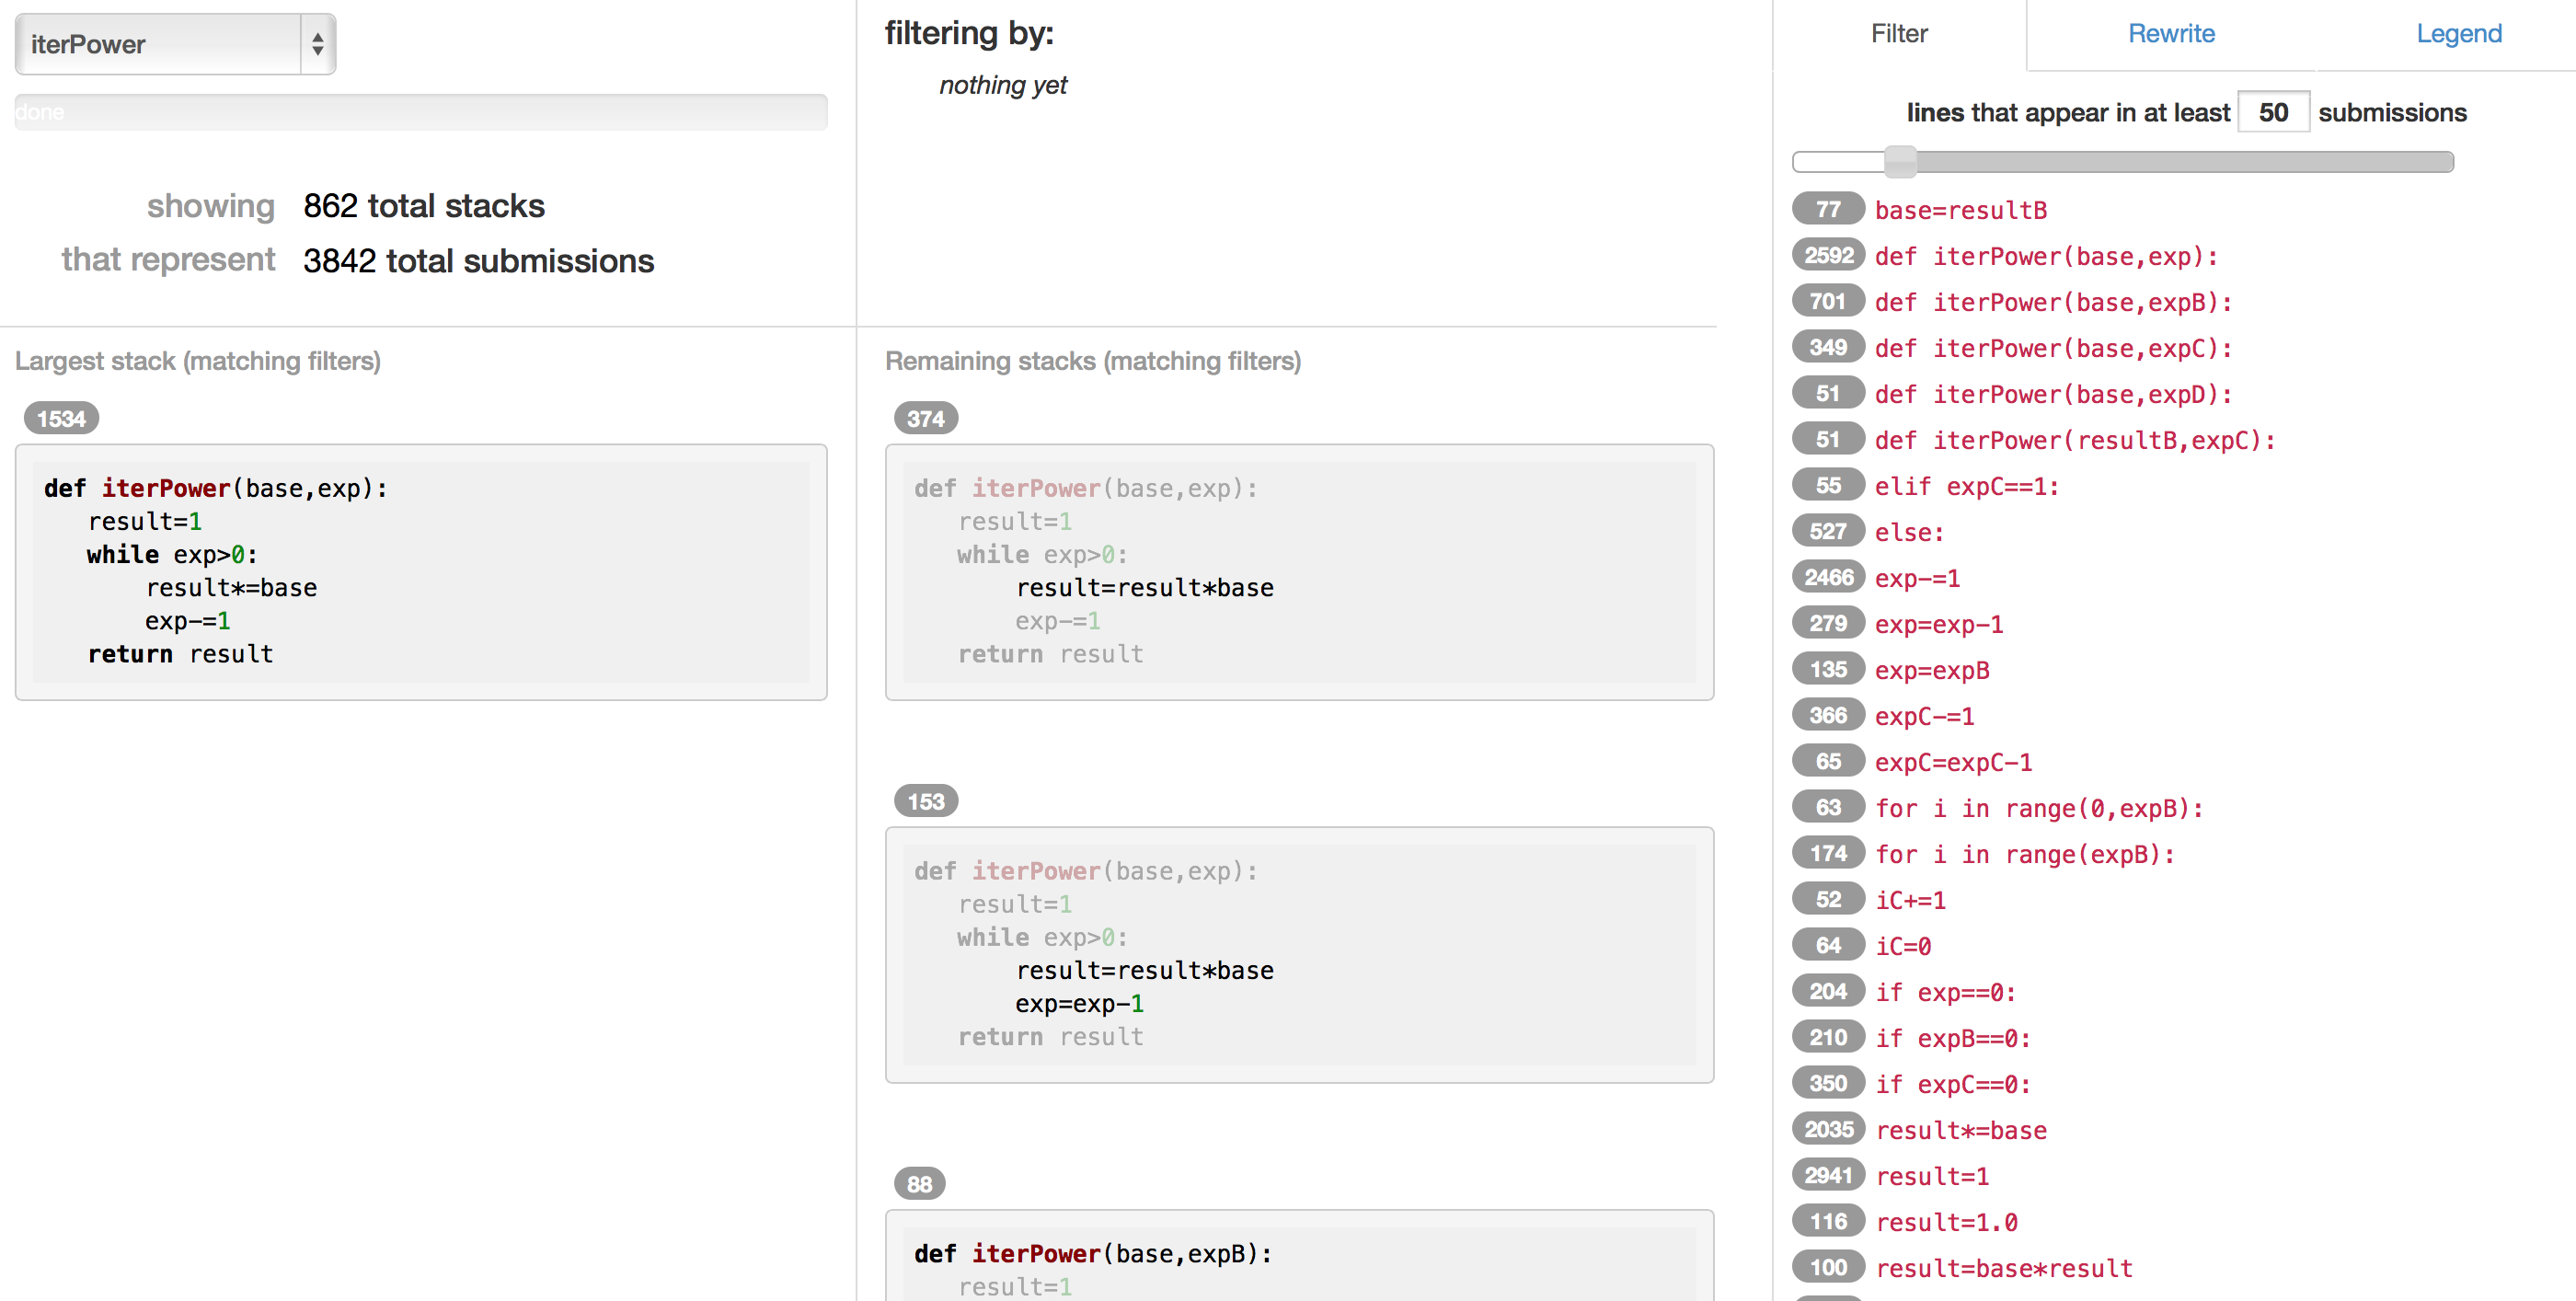
\includegraphics[width=1.0\linewidth]{Body/figures/overcode/interfaceScreenShot.png}
\caption{The OverCode user interface. The top left panel shows the number of clusters, called {\it stacks}, and the total number of solutions visualized. The next panel down in the first column shows the largest stack, while the second column shows the remaining stacks. The third column shows the lines of code in the platonic solutions and their frequencies.}
\label{overcode_fullinterface}
\end{figure*}

Sifting through thousands of solutions to understand their variation and find pedagogically valuable examples is a daunting task, even if the programming problems are simple and the solutions are only tens of lines of code long. Without tool support, a teacher may not read more than 50-100 of them before growing frustrated with the tedium of the task. Given this small sample size, teachers cannot be expected to develop a thorough understanding of the variety of strategies used to solve the problem, produce instructive feedback that is relevant to a large proportion of learners, or find unexpected interesting solutions.

An information visualization approach would enable teachers to explore the variation in solutions at scale. Existing techniques~\cite{gradingsigcse14,MOOCshop,codewebs} use a combination of clustering to group solutions that are semantically similar, and graph visualization to show the variation between these clusters. These clustering algorithms perform pairwise comparisons that are quadratic in both the number of solutions and in the size of each solution, which scales poorly to thousands of solutions. Graph visualization also struggles with how to label the graph node for a cluster, because it has been formed by a complex combination of code features. Without meaningful labels for clusters in the graph, the rich information in student solutions is lost and the teacher's ability to understand variation is weakened.

This chapter presents OverCode, a system for visualizing and exploring the variation in thousands of programming solutions. OverCode is designed to visualize correct solutions, in the sense that they already passed the automatic grading tests typically used in a programming class at scale. The autograder cannot offer any further feedback on these correct solutions, and yet there may still be good and bad variations on correct solutions that are pedagogically valuable to highlight and discuss. OverCode aims to help teachers understand solution variation so that they can provide appropriate feedback to students at scale.

OverCode uses a novel human-interpretable solution clustering technique. The clustering process is linear in time with respect to both the number of solutions and the size of each solution. The platonic solution that represents each cluster is readable, executable, and describes every solution in that cluster in a deterministic way that accounts for both syntax and behavior on test cases. The platonic solutions are shown in a visualization that puts code front-and-center (Figure~\ref{overcode_fullinterface}). In the OverCode interface, teachers read through platonic solutions that each represent entire clusters of solutions. The differences between clusters are highlighted to help teachers discover and understand the variations among solutions. Clusters can be filtered by the lines of code within them.  Clusters can also be merged together with {\em rewrite rules} that collapse variations that the teacher decides are unimportant. 

A cluster in OverCode is a set of solutions that perform the same computations, but may use different variable names or statement order.  OverCode uses a lightweight dynamic analysis to generate clusters, which scales linearly with the number of solutions. It clusters solutions whose variables take the same sequence of values when executed on test inputs and whose set of constituent lines of code are syntactically the same. 

An important component of this analysis is to rename variables that behave the same across different solutions. The renaming of variables serves three main purposes. First, it lets teachers create a mental mapping between variable names and their behavior which is consistent across the entire set of solutions. This may reduce the cognitive load for a teacher to understand different solutions. Second, it helps clustering by reducing variation between similar solutions. Finally, it also helps make the remaining differences between different solutions more salient. 

This chapter concludes by presenting two user studies with a total of 24 participants who each looked at thousands of solutions from an introductory programming MOOC, the OverCode interface is compared with a baseline interface that showed original unclustered solutions. When using OverCode, participants felt that they were able to develop a better high-level view of the students' understandings and misconceptions. While participants didn't necessarily read more lines of code in the OverCode interface than in the baseline, the code they did read came from clusters containing a greater percentage of all the submitted solutions. Participants also drafted mock class forum posts about common good and bad solutions. These forum posts were relevant to more student solutions when using OverCode as compared to the baseline. 

\section{OverCode} \label{overcode}
OverCode is an information visualization application for teachers to explore student solutions. OverCode uses the metaphor of solutions stacked on top of each other to denote a cluster of similar solutions. The top solution in the stack is the platonic solution that represents all the other solutions in the stack. The OverCode interface allows the teacher to scroll through, filter, and merge stacks of solutions. 

The platonic solutions that represent stacks are normalized in a novel way. Specifically, they have standardized formatting, no comments, and variable names that reflect the most popular naming choices across all solutions. They can be filtered by the normalized lines of code they contain and, through rewrite rules, modified and merged. They are the result of the normalization process applied to all student solutions in the OverCode analysis pipeline. %They can also be rewritten when teachers compose and apply \emph{rewrite rules}, which can eliminate differences between platonic solutions and therefore merge stacks that have become identical after the rewrite. 

%The OverCode interface was iteratively designed and developed based on continuous evaluation by the authors, feedback from teachers and peers, and by consulting principles from the information visualization literature. 
A screenshot of OverCode visualizing \codevar{iterPower}, one of the problems from our dataset, is shown in Figure~\ref{overcode_fullinterface}. In this section, the intended use cases and the user interface are described. In Section \ref{pipeline}, the backend program analysis pipeline is described in detail. 
\subsection{Target Users and Tasks}
The target users of OverCode are teaching staff of introductory programming courses. Teaching staff may be undergraduate lab assistants who help students debug their code; graduate students who grade assignments, help students debug, and manage recitations and course forums; and instructors who compose major course assessments. Teachers using OverCode may be looking for common misconceptions, creating a grading rubric, or choosing pedagogically valuable examples to review with students in a future lesson.

\subsubsection{Misconceptions and Holes in Student Knowledge}
Students just starting to learn programming can have a difficult time understanding the language constructs and different API methods. They may use them suboptimally, or in non-standard ways. OverCode may help instructors identify these common misconceptions and holes in knowledge, by highlighting the differences between stacks of solutions. Since the visualized solutions have already been tested and found correct by an autograder, these highlighted differences between platonic solutions may be convoluted variations in construct usage and API method choices that have not been flagged by the Python interpreter or caused the failure of a unit test. Convoluted code may suggest a misconception.

\todo{Rob: it would be great to show example code for these tasks, ideally showing them in OverCode -- can you mine any examples from your thesis defense talk?}

\subsubsection{Grading Rubrics}
It is a difficult task to create grading rubrics for checking properties such as design and style of solutions. Therefore most autograders resort to checking only functional correctness of solutions by testing them against a test suite of input-output pairs. OverCode enables teachers to identify the style, structure, and relative frequency of the variation within correct solutions. Unlike traditional ways of creating a grading rubric, where an instructor may go through a set of solutions, revising the rubric along the way, instructors can use OverCode to first get a high-level overview of the variations before designing a corresponding rubric. Teachers may also see incorrect solutions not caught by the autograder.

\subsubsection{Pedagogically Valuable Examples} 
There can be a variety of ways to solve a given problem and express it in code. If an assignment allows students to generate different solutions, e.g., recursive or iterative, to fulfill the same input-output behavior, OverCode will show separate stacks for each of these different solutions, as well as stacks for every variant of those solutions. OverCode helps teachers filter through solutions to find different examples of solutions to the same problem, which may be pedagogically valuable. According to variation theory ~\cite{marton13}, students can learn through concrete examples of these multiple solutions, which vary along different conceptual dimensions.
\subsection{User Interface}

The OverCode user interface is the product of an iterative design process with multiple stages, including paper prototypes and low-fidelity prototypes rendered in a web browser.  Prototype iterations were used and critiqued by members of our research group and by several teaching staff of an introductory Python programming course. While exploring the low-fidelity prototypes, these teachers talked aloud about their hopes for what the tool could do, frustrations with its current form, and their frustrations with existing solution-viewing tools and processes. This feedback was incorporated into the final design.

The OverCode user interface is divided into three columns. The top-left panel in the first column shows the problem name, the \emph{done} progress bar, the number of stacks, the number of visualized stacks given the current filters and rewrite rules, and the total number of solutions those visualized stacks contain. The panel below shows the largest stack of solutions. Side by side with the largest stack, the remaining stacks appear in the second panel. Through scrolling, any stack can be horizontally aligned with the largest stack for easier comparison. The third panel has three different tabs that provide static and dynamic information about the solutions, and the ability to filter and combine stacks. 

As shown in Figure~\ref{overcode_fullinterface}, the default tab shows a list of lines of code that occur in different platonic solutions together with their corresponding frequencies. The stacks can be filtered based on the occurrence of one or more lines (Filter tab). The column also has tabs for \emph{Rewrite} and \emph{Legend}. The Rewrite tab allows a teacher to provide rewrite rules to collapse different stacks with small differences into a larger single stack. The Legend tab shows the dynamic values that different program variables take during the execution of programs over a test case. %We now describe different features of OverCode in more detail.
\todo{ROB:maybe the TOCHI paper didn't have space for screenshots of these, but your thesis needs them}

\subsubsection{Stacks} A stack in OverCode denotes a set of similar solutions that are grouped together based on a similarity criterion defined in Section \ref{pipeline}. For example, a stack for the \codevar{iterPower} problem is shown in Figure~\ref{stacks}(a). The size of each stack, i.e., the number of solutions in a stack, is shown in a pillbox at the top-left corner of the stack. Stacks are listed in the scrollable second panel from largest to smallest. The solution on the top of the stack is a platonic solution that describes all the solutions in the stack. See Section \ref{pipeline} for details on the normalizing process that produces platonic solutions.

Each stack can also be clicked. After clicking a stack, the border color of the stack changes and the \emph{done} progress bar is updated to reflect the percentage of total solutions clicked, as shown in Figure~\ref{stacks}(b). This feature is intended to help teachers remember which stacks they have already read or analyzed, and keep track of their progress. Clicking on a large stack, which represents a significant fraction of the total solutions, is reflected by a large change in the \emph{done} progress bar. \todo{add that now the raw solutions inside the stack are also displayed, but this was not included during user study tests}

\begin{figure*}[htpb]
\begin{tabular}{c | c}
\begin{minipage}{.5\linewidth}
\centering
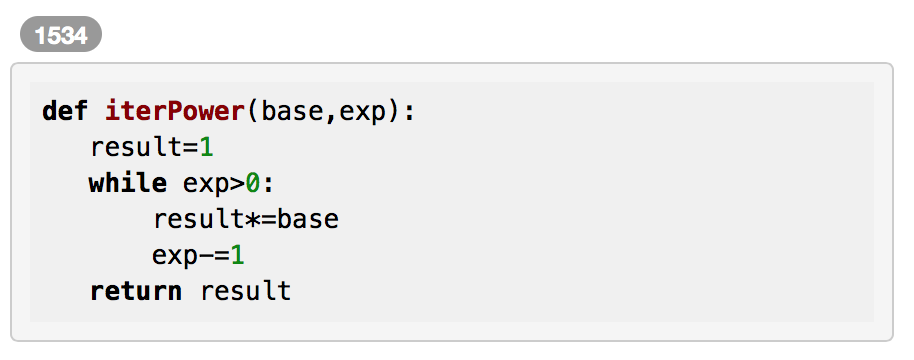
\includegraphics[width=0.95\linewidth]{Body/figures/overcode/stackScreenShot.png}
\end{minipage}
&
\begin{minipage}{.5\linewidth}
\centering
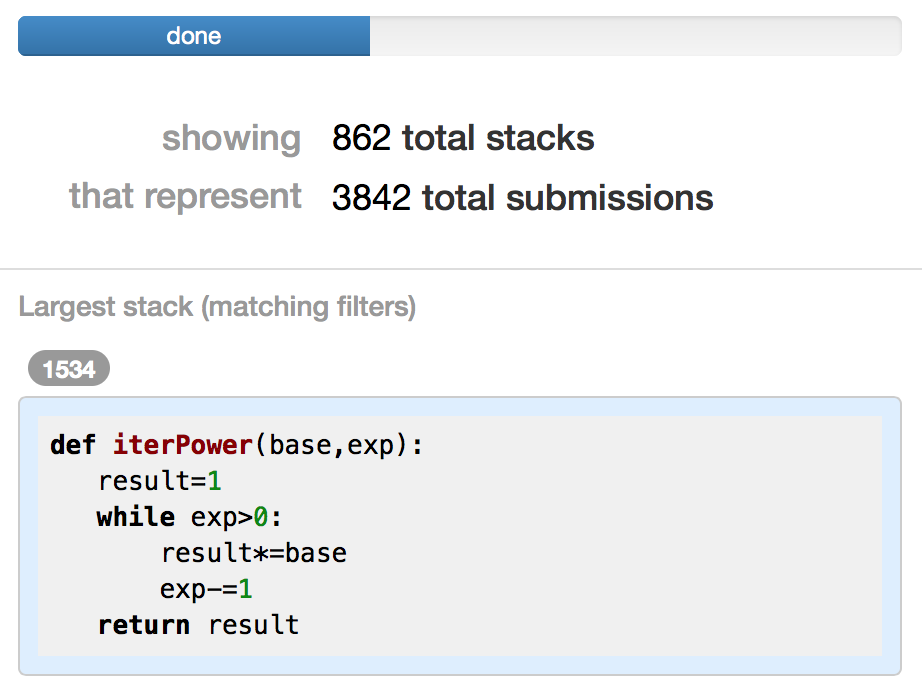
\includegraphics[width=0.95\linewidth]{Body/figures/overcode/checkDone.png}
\end{minipage}
\\
(a) & (b)
\end{tabular}
\caption{(a) A stack of 1534 similar \codevar{iterPower} solutions. (b) After clicking a stack, the border color of the stack changes and the done progress bar denotes the corresponding fraction of solutions that have been checked.}
\label{stacks}
\end{figure*}

\subsubsection{Showing Differences between Stacks} OverCode allows teachers to compare smaller stacks, shown in the second column, with the largest stack, shown in the first column. The lines of code in the second column that also appear in the set of lines in the largest stack are dimmed so that only the differences between the smaller stacks and the largest stack are apparent. For example, Figure~\ref{stackdifferences} shows the differences between the platonic solutions of the two largest stacks. In earlier iterations of the user interface, lines in stacks that were not shared with the largest stack were highlighted in yellow, but this produced a lot of visual noise. By dimming the lines in stacks that \textit{are} shared with the largest stack, the visible noise is reduced, while still keeping differences between stacks salient.

\begin{figure*}
\centering
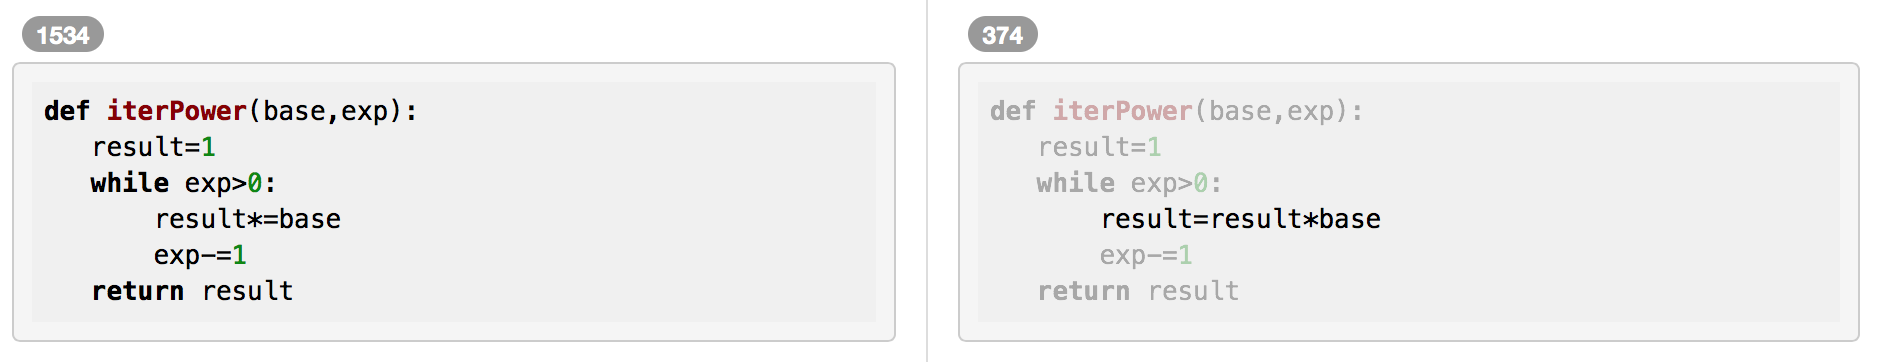
\includegraphics[scale=0.42]{Body/figures/overcode/lineFadingScreenshot}
\caption{Similar lines of code between two stacks are dimmed out such that only differences between the two stacks are apparent.}
\label{stackdifferences}
\end{figure*}



\subsubsection{Filtering Stacks by Lines of Code} The third column of OverCode shows the list of lines of code occurring in the solutions together with their frequencies (numbered pillboxes). The interface has a slider that can be used to change the threshold value, which denotes the number of solutions in which a line should appear for it to be included in the list. For example, by dragging the slider to $200$ in Figure~\ref{linefilter}(a), OverCode only shows lines of code that are present in at least $200$ solutions. This feature was added as a response to the length of the unfiltered list of code lines, which was long enough to make skimming for common code lines difficult.

Users can filter the stacks by selecting one or more lines of code from the list. After each selection, only stacks whose platonic solutions have those selected lines of code are shown. Figure~\ref{linefilter}(b) shows a filtering of stacks that have a \codevar{for} loop, specifically the line of code \codevar{for i in range(expB)}, and that assign $1$ to the variable \codevar{result}.

\begin{figure*}[htpb]
\begin{tabular}{c | c}
\begin{minipage}{.48\linewidth}
\centering
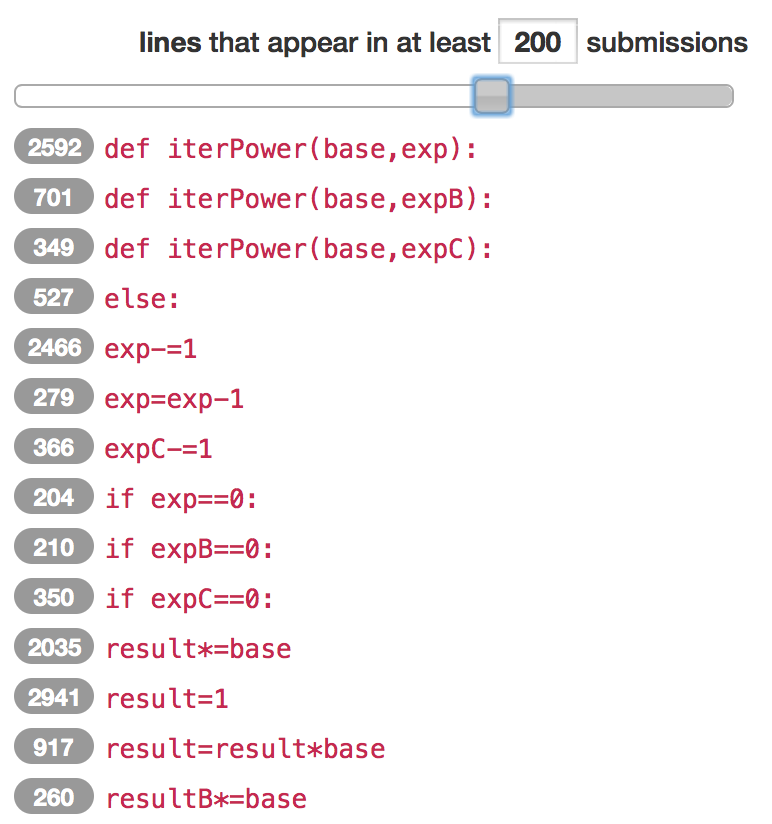
\includegraphics[scale=0.5]{Body/figures/overcode/lineSlider.png}
\end{minipage}
&
\begin{minipage}{.52\linewidth}
\centering
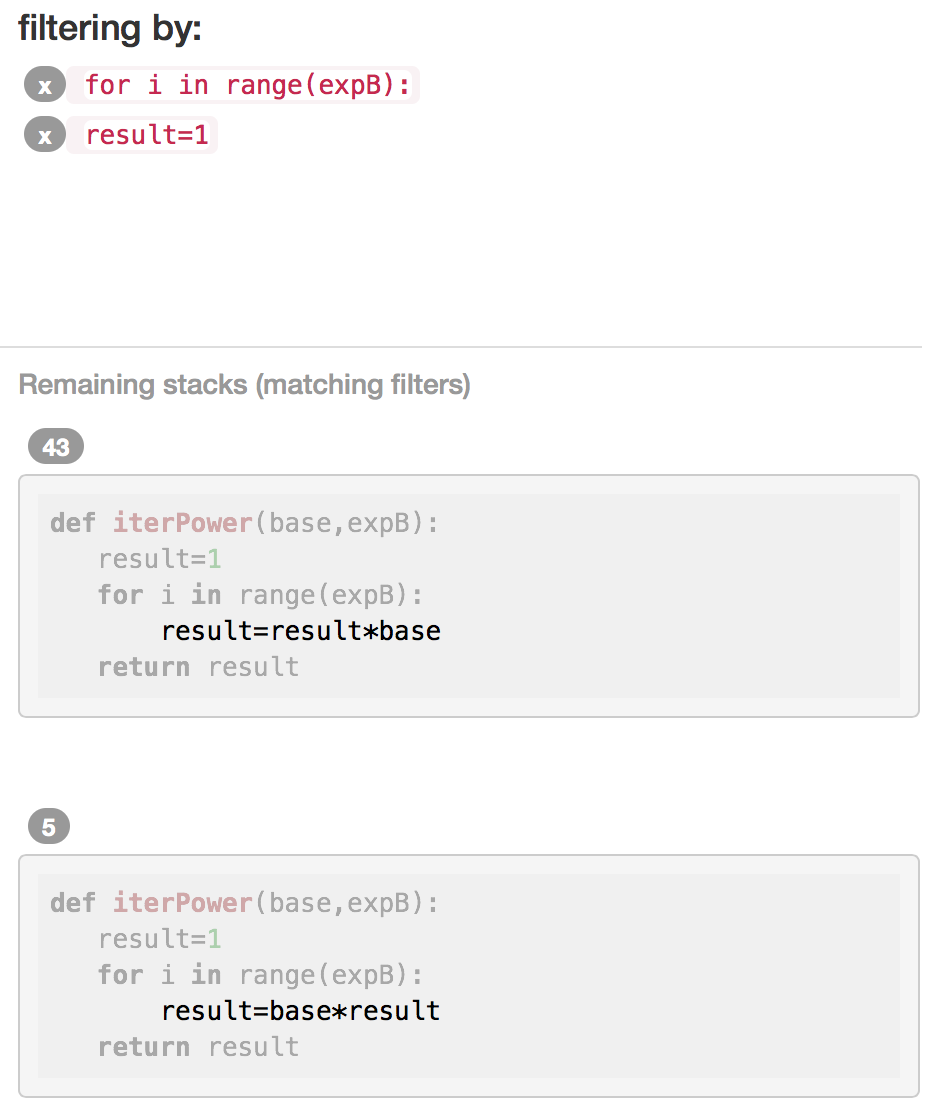
\includegraphics[scale=0.40]{Body/figures/overcode/lineFilter.png}
\end{minipage}
\\
(a) & (b)
\end{tabular}
\caption{(a) The slider allows filtering of the list of lines of code by the number of solutions in which they appear. (b) Clicking on a line of code adds it to the list of lines by which the stacks are filtered.}
\label{linefilter}
\end{figure*}

\subsubsection{Rewrite Rules} There are often small differences between the platonic solutions that can lead to a large number of stacks for a teacher to review. OverCode provides \emph{rewrite rules} by which teachers can collapse these differences and ignore variation they do not need to see. This feature comes from experience with early prototypes. After observing a difference between stacks, like the use of \codevar{xrange} instead of \codevar{range}, teachers wanted to ignore that difference in order to more easily find other differences.

A rewrite rule is described with a left hand side and a right hand side as shown in Figure~\ref{rewriterule}(a). The semantics of a rewrite rule is to replace all occurrences of the left-hand side expression in the platonic solutions with the corresponding right-hand side. As the rewrite rules are entered, OverCode presents a preview of the changes in the platonic solutions as shown in Figure~\ref{rewriterule}(b). After the application of the rewrite rules, OverCode collapses stacks that now have the same platonic solutions because of the rewrites. For example, after the application of the rewrite rule in Figure~\ref{rewriterule}(a), OverCode collapses the two biggest iterPower stacks from Figure~\ref{overcode_fullinterface} of sizes $1534$ and $374$, respectively, into a single stack of size $1908$. Other pairs of stacks whose differences have now been removed by the rewrite rule are also collapsed into single stacks. As shown in Figure~\ref{afterrewrite}(a), the number of stacks now drop from $862$ to $814$.

\begin{figure*}[htpb]
\begin{tabular}{c | c}
\begin{minipage}{.5\linewidth}
\centering
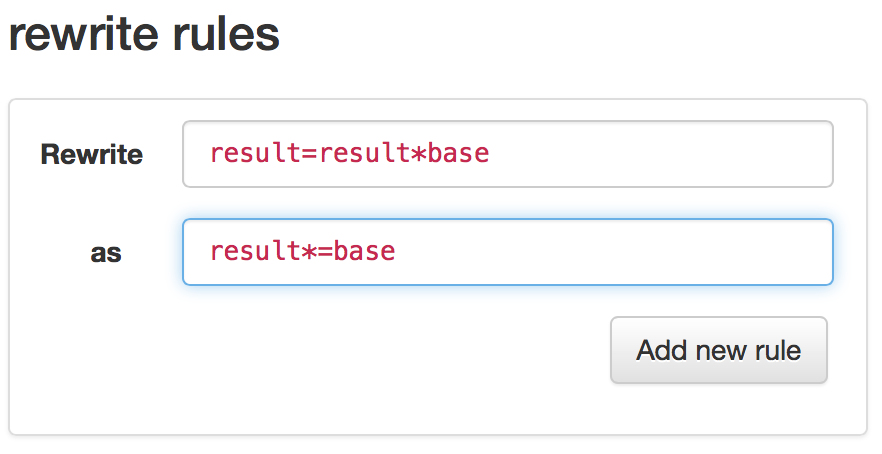
\includegraphics[scale=0.45]{Body/figures/overcode/rewriteRuleScreenshot.png}
\end{minipage}
&
\begin{minipage}{.5\linewidth}
\centering
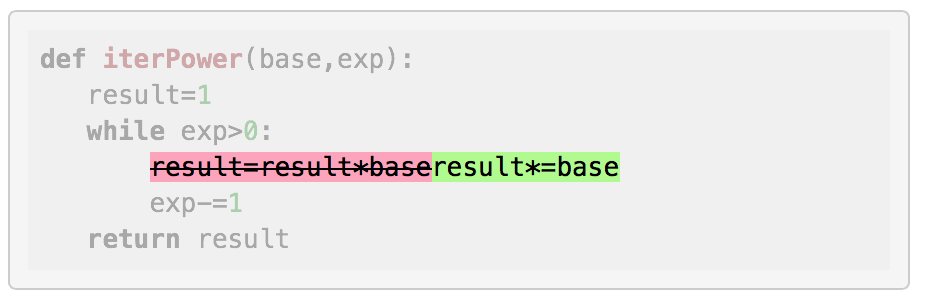
\includegraphics[scale=0.40]{Body/figures/overcode/rewritePreviewScreenShot.png}
\end{minipage}
\\
(a) & (b)
\end{tabular}
\caption{(a) An example rewrite rule to replace all occurrences of statement \codevar{result = base * result} with \codevar{result *= base}. (b) The preview of the changes in the platonic solutions because of the application of the rewrite rule.}
\label{rewriterule}
\end{figure*}

\begin{figure*}[htpb]
\begin{tabular}{c | c}
\begin{minipage}{.5\linewidth}
\centering
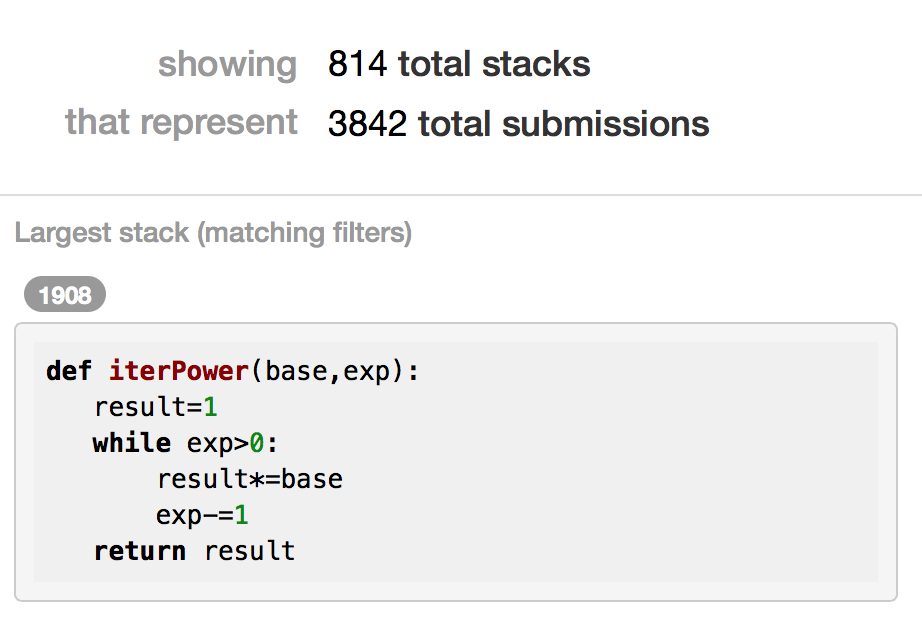
\includegraphics[scale=0.4]{Body/figures/overcode/afterrewrite.png}
\end{minipage}
&
\begin{minipage}{.5\linewidth}
\centering
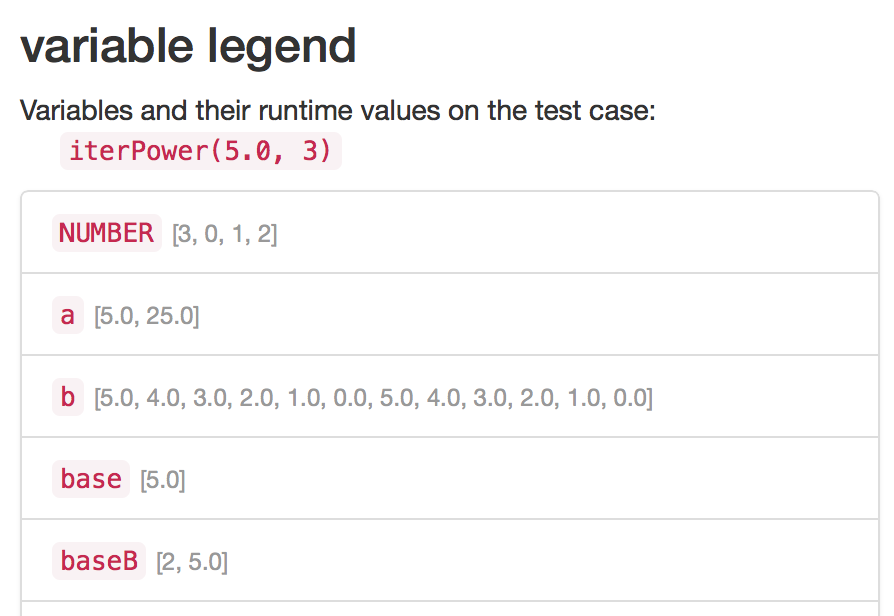
\includegraphics[scale=0.4]{Body/figures/overcode/variableLegend.png}
\end{minipage}
\\
(a) & (b)
\end{tabular}
\caption{(a) The merging of stacks after application of the rewrite rule shown in Figure~\ref{rewriterule}. (b) The variable legend shows the sequence of dynamic values that all program variables in normalized solutions take over the course of execution on a given test case.}
\label{afterrewrite}
\end{figure*}

\subsubsection{Variable Legends} OverCode also shows the sequence of values that variables in the platonic solutions take on, over the course of their execution on a test case. As described in Section~\ref{pipeline}, a variable is identified by the sequence of values it takes on during the execution of the test case. Figure~\ref{afterrewrite}(b) shows a snapshot of the variable values for the \codevar{iterPower} problem. The goal of presenting this dynamic information associated with common variable names is intended to help teachers (1) understand the behavior of each platonic solution without having to mentally execute it on a test case and (2) further explore the variations among solutions that do not have the same common variables. When this legend was originally added to the user interface, clicking on a common variable name would filter for all solutions that contained an instance of that variable. Some pilot users found this feature confusing, rather than empowering. As a result, it was removed from OverCode before running both user studies. At least one study participant, upon realizing the value of the legend, wished that the original click-to-filter-by-variable functionality existed; it may be reinstated in future versions.

\section{Implementation} \label{pipeline}
The OverCode user interface depends on an analysis pipeline that normalizes solutions in a manner designed for human readability. The pipeline then creates stacks of solutions that have become identical through the normalizing process. The pipeline accepts, as input, a set of solutions, expressed as function definitions for $f(a,...)$, and a set of test cases. Solutions that enter the pipeline are referred to as \emph{raw}, and the solutions that exit the pipeline as \emph{normal}. Examples, beginning with \codevar{iterPower}, are presented below to illustrate this pipeline.

\subsection{Analysis Pipeline}
OverCode is currently implemented for Python, but the pipeline steps described below could be readily generalized to other languages commonly used to teach programming.

{\bf 1. Reformat solutions.} For a consistent appearance, the solutions are reformatted with the PythonTidy package\footnote{Created by Charles Curtis Rhode. \url{https://pypi.python.org/pypi/PythonTidy/}} to have consistent line indentation and token spacing. Comments and empty lines are also removed. These steps not only make solutions more readable, but also allow exact string matches between solutions, after additional normalizing steps later in the pipeline. Although comments can contain valuable information, the variation in comments is so great that clustering and summarizing them will require significant additional design, which remains future work. Figure~\ref{fig:reformat} illustrates the effect of this reformatting.
\begin{figure}
\begin{tabular}{ll}
{\bf Student A Raw Code} & {\bf Student A Reformatted} \\
\begin{minipage}{0.5\linewidth}
\begin{lstlisting}[basicstyle=\linespread{1.0}\ttfamily\footnotesize,language=python]
def iterPower(base, exp):
    '''
    base: int or float.
    exp: int >= 0
    returns: int or float, base^exp
    '''
    result = 1
    for i in range(exp):
        result *= base
    return result
\end{lstlisting}
\end{minipage}
&
\begin{minipage}{0.5\linewidth}
\begin{lstlisting}[basicstyle=\linespread{1.0}\ttfamily\footnotesize,language=python]
def iterPower(base,exp):
    result=1
    for i in range(exp):
        result*=base
    return result
\end{lstlisting}
\end{minipage}
\end{tabular}
\caption{A student solution before and after reformatting.}
\label{fig:reformat}
\end{figure}

{\bf 2. Execute solutions.} Each solution is on the same test case(s). During each step of the execution for each test case, the names and values of local and global variables, and also return values from functions, are recorded as a program trace using an adaptation of Philip Guo's logger~\cite{pgbovineOPT}. There is one program trace per solution per test case. Included for the purpose of illustrating this pipeline, the examples in the figures that follow are derived from executing definitions of \codevar{iterPower} on a \codevar{base} of $5.0$ and an \codevar{exp} of $3$, as illustrated in Figure~\ref{fig:testcase}.
\begin{figure}
\begin{tabular}{l}
{\bf Student Code with Test Case} \\
\begin{minipage}{0.5\linewidth}
\begin{lstlisting}[basicstyle=\linespread{1.0}\ttfamily\footnotesize,language=python]
def iterPower(base,exp):
    #student code here
iterPower(5.0, 3)
\end{lstlisting}
\end{minipage} 
\end{tabular}
\caption{Illustration of running a (dummy) \texttt{iterPower} solution on a test case.}
\label{fig:testcase}
\end{figure}

{\bf 3. Extract variable sequences.} For each variable in a program trace, the pipeline extracts the sequence of distinct values it takes on. Figure~\ref{fig:extractsequence} shows the program trace for a solution run on a test case, as well as the extracted sequences of distinct values for each variable. Variable sequence extraction also works for purely functional programs, in which variables are never reassigned, because each recursive invocation is treated as if new values are given to its parameter variables. For example, in spite of the fact that the \codevar{iterPower} problem asked students to compute the exponential $\codevar{base}^\codevar{exp}$ \textit{iteratively}, $60$ of the $3842$ \codevar{iterPower} solutions in the dataset were in fact recursive. One of these recursive examples is shown in Figure~\ref{fig:recursiveTrace}, along with the variable sequences extracted.
\begin{figure}
\begin{tabular}{ll}
{\bf Student A Code with Test Case} & {\bf Program Trace for Student A Code} \\
\begin{minipage}{0.35\linewidth}
\begin{lstlisting}[basicstyle=\linespread{1.0}\ttfamily\footnotesize,language=python]
def iterPower(base,exp):
    result=1
    for i in range(exp):
        result*=base
    return result
iterPower(5.0, 3)
\end{lstlisting}
\end{minipage} &
\begin{minipage}{0.6\linewidth}
\begin{lstlisting}[basicstyle=\linespread{1.0}\ttfamily\footnotesize,language=python,linebackgroundcolor={\lstcolorlines[gray!20]{2,4,6,8,10,12,14,16,18}}]
iterPower(5.0, 3)
 base : 5.0, exp : 3
result=1
 base : 5.0, exp : 3, result : 1 
for i in range(exp):
 base : 5.0, exp : 3, result : 1, i : 0
result*=base
 base : 5.0, exp : 3, result : 5.0, i : 0 
for i in range(exp):
 base : 5.0, exp : 3, result : 5.0, i : 1
result*=base 
 base : 5.0, exp : 3, result : 25.0, i : 1 
for i in range(exp):
 base : 5.0, exp : 3, result : 25.0, i : 2 
result*=base
 base : 5.0, exp : 3, result : 125.0, i : 2
return result
 value returned: 125.0
\end{lstlisting}
\end{minipage} 
\\
& {\bf Variable Sequences for Student A Code} \\
&
\begin{minipage}{0.6\linewidth}
\begin{lstlisting}[language=python]
base: 5.0
exp: 3
result: 1, 5.0, 25.0, 125.0
i: 0, 1, 2
\end{lstlisting}
\end{minipage}
\end{tabular}
\caption{A student solution, its program trace when running on the test case \texttt{iterPower(5.0,3)}, and the sequence of values extracted from the trace for each variable.}
\label{fig:extractsequence}
\end{figure}

\begin{figure}
\begin{tabular}{ll}
{\bf Recursive Example} & {\bf Program Trace} \\
 % & {\bf for Recursive Example} \\
\begin{minipage}{0.5\linewidth}
\begin{lstlisting}[basicstyle=\linespread{1.0}\ttfamily\footnotesize,language=python]
def iterPower(base,exp):
   if exp==0:
       return 1
   else:
       return base*iterPower(base,exp-1)
iterPower(5.0, 3)
\end{lstlisting}
\end{minipage} &
\begin{minipage}{0.4\linewidth}
\begin{lstlisting}[basicstyle=\linespread{1.0}\ttfamily\footnotesize,language=python,linebackgroundcolor={\lstcolorlines[gray!20]{2,4,6,8,10,12,14,16,18,20,22,24,26,28,30}}]
iterPower(5.0, 3)
 base : 5.0, exp : 3
if exp==0:
 base : 5.0, exp : 3 
return base*iterPower(base,exp-1)
 base : 5.0, exp : 3 
iterPower(5.0, 2)
 base : 5.0, exp : 2
if exp==0: 
 base : 5.0, exp : 2 
return base*iterPower(base,exp-1)
 base : 5.0, exp : 2
iterPower(5.0, 1)
 base : 5.0, exp : 1
if exp==0:
 base : 5.0, exp : 1
return base*iterPower(base,exp-1)
 base : 5.0, exp : 1
iterPower(5.0, 0)
 base : 5.0, exp : 0
if exp==0:
 base : 5.0, exp : 0
return 1
 base : 5.0, exp : 0
return base*1
 base : 5.0, exp : 1
return base*5
 base : 5.0, exp : 2
return base*25
 base : 5.0, exp : 3
value returned: 125.0
\end{lstlisting}
\end{minipage} 
\\
& {\bf Variable Sequences} \\
% & {\bf for Recursive Example} \\
&
\begin{minipage}{0.5\linewidth}
\begin{lstlisting}[language=python]
base: 5.0
exp: 3, 2, 1, 0, 1, 2, 3
\end{lstlisting}
\end{minipage}
\end{tabular}
\caption{A recursive solution to the same programming problem, its program trace when executing on \texttt{iterPower(5.0,3)}, and the extracted sequences of values for each variable.}
\label{fig:recursiveTrace}
\end{figure}


{\bf 4. Identify common variables.} The pipeline analyzes all program traces, identifying which variables' sequences are identical. Variables that have identical sequences across two or more program traces are referred to as {\it common variables}. Variables which occur in only one program trace are called {\it unique variables}. This is illustrated in Figures~\ref{fig:commik} and~\ref{fig:allvars}.
\begin{figure}
\begin{tabular}{ll}
{\bf Student B Code with Test Case} & {\bf Variable Sequences for Student B Code} \\
\begin{minipage}{0.5\linewidth}
\begin{lstlisting}[basicstyle=\linespread{1.0}\ttfamily\footnotesize,language=python]
def iterPower(base,exp):
    r=1
    for k in xrange(exp):
        r=r*base
    return r
iterPower(5.0, 3)
\end{lstlisting}
\end{minipage}
&
\begin{minipage}{0.5\linewidth}
\begin{lstlisting}[language=python]
base: 5.0
exp: 3
r: 1, 5.0, 25.0, 125.0
k: 0, 1, 2
\end{lstlisting}
\end{minipage} \\
{\bf Student C Code with Test Case} & {\bf Variable Sequences for Student C Code} \\
\begin{minipage}{0.5\linewidth}
\begin{lstlisting}[basicstyle=\linespread{1.0}\ttfamily\footnotesize,language=python]
def iterPower(base,exp):
   result=1
   while exp>0:
       result*=base
       exp-=1
   return result
iterPower(5.0, 3)
\end{lstlisting}
\end{minipage}
&
\begin{minipage}{0.5\linewidth}
\begin{lstlisting}[language=python]
base : 5.0
exp: 3
result : 1, 5.0, 25.0, 125.0
exp : 3, 2, 1, 0
\end{lstlisting}
\end{minipage}
\end{tabular}
\caption{\codevar{i} and \codevar{k} take on the same sequence of values in Student A's and Student B's code: $0$,$1$,$2$. They are therefore considered the same {\it common variable}.}
\label{fig:commik}
\end{figure}
\begin{figure}
{\bf Common variables} in Students A, B, and C's code:
\begin{itemize}
\item \texttt{5.0}:
\begin{itemize}
\item \texttt{base} (Students A, B, C)
\end{itemize}
\item \texttt{3}:
\begin{itemize}
\item \texttt{exp} (Students A, B) 
\end{itemize}
\item \texttt{1, 5.0, 25.0, 125.0}: 
\begin{itemize}
\item \texttt{result} (Students A, C)
\item \texttt{r} (Student B)
\end{itemize}
\item \texttt{0,1,2}:
\begin{itemize}
\item \texttt{i} (Student A) 
\item \texttt{k} (Student B)
\end{itemize}
\end{itemize}
{\bf Unique variables} in Students A, B, and C's code:
\begin{itemize}
\item \texttt{3,2,1,0}:
\begin{itemize}
\item \texttt{exp} (Student C)
\end{itemize}
\end{itemize}
\caption{Common and uncommon variables found across the solutions in the previous figure.}
\label{fig:allvars}
\end{figure}

{\bf 5. Rename common and unique variables.} A common variable may have a different name in each program trace. In this step, the common variable is renamed to the name that is given most often to that common variable across all program traces. 

There are exceptions made to avoid name collisions. For example, the unique variable in the previous pipeline step was originally named \codevar{exp}. As shown in Figure~\ref{fig:uniqcomm}, OverCode appends a double underscore as a modifier to resolve a name collision with the common variable of the same name. This is referred to as a unique/common collision.
\begin{figure}
\begin{tabular}{ll}
{\bf Common Variables, Named} & {\bf Unique Variables, Named} \\
\begin{minipage}{0.5\linewidth}
\begin{itemize}
\item \texttt{base: 5.0} 
\item \texttt{exp: 3} 
\item \texttt{result: 1, 5.0, 25.0, 125.0}
\item \texttt{i: 0,1,2} (common name tie broken by random choice)
\end{itemize}
\end{minipage}
&
\begin{minipage}{0.5\linewidth}
\begin{itemize}
\item \begin{verbatim} exp__: 3,2,1,0 \end{verbatim}
\end{itemize}
\end{minipage}

\end{tabular}
\caption{The unique variable in the previous pipeline step was originally named \codevar{exp}. OverCode appends a double underscore as a modifier to resolve a name collision with the common variable of the same name. This is referred to as a unique/common collision.}
\label{fig:uniqcomm}
\end{figure}

After common and unique variables in the solutions are renamed, the solutions are now called {\it normal}, as shown in Figure~\ref{fig:normalcode}.
\begin{figure}
\begin{tabular}{ll}

{\bf Normal Student A Code} & {\bf Normal Student B Code} \\ 

\begin{minipage}{0.5\linewidth}
\begin{lstlisting}[basicstyle=\linespread{1.0}\ttfamily\footnotesize,language=python]
def iterPower(base,exp):
    result=1
    for i in range(exp):
        result*=base
    return result
\end{lstlisting}
\end{minipage} &
\begin{minipage}{0.5\linewidth}
\begin{lstlisting}[basicstyle=\linespread{1.0}\ttfamily\footnotesize,language=python]
def iterPower(base,exp):
    result=1
    for i in xrange(exp):
        result=result*base
    return result
\end{lstlisting}
\end{minipage}
\\
{\bf Normal Student C Code} &  \\
\begin{minipage}{0.5\linewidth}
\begin{lstlisting}[basicstyle=\linespread{1.0}\ttfamily\footnotesize,language=python]
def iterPower(base,exp__):
   result=1
   while exp__>0:
       result*=base
       exp__-=1
   return result
\end{lstlisting}
\end{minipage}
& \\
\end{tabular}
\caption{Normalized solutions after variable renaming.}
\label{fig:normalcode}
\end{figure}

{\bf 6. Make stacks.} The pipeline iterates through the normal solutions, making stacks of solutions that share an identical {\it set} of lines of code. The pipeline compares sets of lines of code because then solutions with arbitrarily ordered lines that do not depend on each other can still fall into the same stack. (Recall that the variables in these lines of code have already been renamed based on their dynamic behavior, and all the solutions have already been marked input-output correct by an autograder, prior to this pipeline.) The platonic solution that represents the stack is randomly chosen from within the stack, because all the normal solutions within the stack are identical, with the possible exception of the order of their statements. 

In the examples in Figure~\ref{fig:makingstacks}, the normal C and D solutions have the same set of lines, and both provide correct output, with respect to the autograder. Therefore, the difference in order of the statements between the two solutions is not communicated to the teacher. The two solutions are put in the same stack, with one solution arbitrarily chosen as the visible normalized code. However, since Student A and Student B use different functions, i.e., \codevar{xrange} vs. \codevar{range}, and different operators, i.e., \codevar{*=} vs. \codevar{=,*}, the pipeline puts them in separate stacks.
%\vspace{10mm}
\begin{figure}
\begin{tabular}{l|l}
{\bf Stack 1} Normal Student A & {\bf Stack 2} Normal Student B  \\
\begin{minipage}{0.5\linewidth}
\begin{lstlisting}[basicstyle=\linespread{1.0}\ttfamily\footnotesize,language=python,linebackgroundcolor={\lstcolorlines[gray!20]{3,4}}]
def iterPower(base,exp):
    result=1
    for i in range(exp):
        result*=base
    return result
\end{lstlisting}
\end{minipage}
&
\begin{minipage}{0.5\linewidth}
\begin{lstlisting}[basicstyle=\linespread{1.0}\ttfamily\footnotesize,language=python,linebackgroundcolor={\lstcolorlines[gray!20]{3,4}}]
def iterPower(base,exp):
    result=1
    for i in xrange(exp):
        result=result*base
    return result
\end{lstlisting}
\end{minipage}
\end{tabular}
\begin{tabular}{ll}
\hline
\\
{\bf Stack 3} Normal Student C & {\bf Stack 3} Normal Student D  \\
\begin{minipage}{0.5\linewidth}
\begin{lstlisting}[basicstyle=\linespread{1.0}\ttfamily\footnotesize,language=python,linebackgroundcolor={\lstcolorlines[mygray]{4,5}}]
def iterPower(base,exp__):
    result=1
    while exp__>0:
        result=result*base
        exp__-=1
    return result
\end{lstlisting}
\end{minipage}
&
\begin{minipage}{0.5\linewidth}
\begin{lstlisting}[basicstyle=\linespread{1.0}\ttfamily\footnotesize,language=python,linebackgroundcolor={\lstcolorlines[mygray]{4,5}}]
def iterPower(base,exp__):
    result=1
    while exp__>0:
        exp__-=1
        result=result*base
    return result
\end{lstlisting}
\end{minipage}
\end{tabular}
\caption{Four solutions collapsed into three stacks.}
\label{fig:makingstacks}
\end{figure}
Some programming problems have no deadline, and new solutions are submitted intermittently. The entire pipeline does not need to be rerun to normalize a new solution and restack all the solutions in the dataset. The pipeline has been split into two phases: solution preprocessing and batch processing. During preprocessing, each solution formatting is standardized and all comments are removed. It is then executed on one or more test cases, which makes the resulting normalization more robust to any individual poorly chosen test case. The full program trace and output is recorded for every test case. 

This logging of solution execution can be one of the longer steps in the OverCode analysis pipeline, so preprocessing occurs once per solution and is saved in its own pickle file. New solutions can be preprocessed once, without affecting previously preprocessed solutions. Batch processing takes, as input, all the existing preprocessed results and normalizes variable names. This must occur as a batch operation because variable renaming depends on the behavior and name of every variable in every solution.

The program tracing \cite{pgbovineOPT} and renaming scripts occasionally generate errors while processing a solution. For example, the script may not have code to handle a particular but rare Python construct. Errors thrown by the scripts drive their development and are helpful for debugging. When errors occur while processing a particular solution, they are excluded from our analysis. Less than five percent of the solutions in each of the three problem datasets are excluded.

\subsection{Variable Renaming Details and Limitations} \label{repercussions}

There are three distinct types of name collisions possible when renaming variables to be consistent across multiple solutions. The first, referred to here as a {\it common/common} collision, occurs when two common variables (with different variable sequences) have the same common name. The second, referred to here as a {\it multiple instances} collision, occurs when there are multiple different instances of the same common variable in a solution. The third and final collision, referred to as a {\it unique/common} collision, occurs when a unique variable's name collides with a common variable's name.

{\bf Common/common collision.} If common variables $cv_{1}$ and $cv_{2}$ are both most frequently named $i$ across all program traces, the pipeline appends a modifier to the name of the less frequently used common variable. For example, if 500 program traces have an instance of $cv_{1}$ and only 250 program traces have an instance of $cv_{2}$, $cv_{1}$ will be named $i$ and $cv_{2}$ will be named $iB$.  

For example, a subset of \codevar{iterPower} solutions created a variable that iterated through the values generated by \codevar{range(exp)}. Student A's code is an example. A smaller subset created a variable that iterated through the values generated by \codevar{range(1,exp+1)}, as seen in Student E's code. These are two separate common variables in our pipeline, due to their differing value sequences. The {\it common/common} name collision arises because both common variables are most frequently named \codevar{i} across all solutions to \codevar{iterPower}. To preserve the one-to-one mapping of variable name to value sequence across the entire \codevar{iterPower} problem dataset, the pipeline appends a modifier, \codevar{B}, to the common variable \codevar{i} found in fewer \codevar{iterPower} solutions. A common variable, also most commonly named \codevar{i}, which is found in even fewer \codevar{iterPower} definitions, will have a \codevar{C} appended, etc. This is illustrated in Figure~\ref{fig:commcommcoll}.
\begin{figure}
\begin{tabular}{l|l}

{\bf Student A (Represents 500 Solutions)} & {\bf Student E (Represents 250 Solutions)} \\
\begin{minipage}{0.5\linewidth}
\begin{lstlisting}[basicstyle=\linespread{1.0}\ttfamily\footnotesize,language=python]
def iterPower(base,exp):
    result=1
    for i in range(exp):
        result*=base
    return result
\end{lstlisting}
\end{minipage}
&
\begin{minipage}{0.5\linewidth}
\begin{lstlisting}[basicstyle=\linespread{1.0}\ttfamily\footnotesize,language=python,linebackgroundcolor={\lstcolorlines[gray!20]{3}}]
def iterPower(base,exp):
   result=1
   for i in range(1,exp+1):
       result*=base
   return result
\end{lstlisting}
\end{minipage}
\\
{\bf Normal Student A (After Renaming)} & {\bf Normal Student E (After Renaming)} \\
\codevar{(unchanged)} 
&
\begin{minipage}{0.5\linewidth}
\begin{lstlisting}[basicstyle=\linespread{1.0}\ttfamily\footnotesize,language=python,linebackgroundcolor={\lstcolorlines[gray!20]{3}}]
def iterPower(base,exp):
   result=1
   for iB in range(1,exp+1):
       result*=base
   return result
\end{lstlisting}
\end{minipage}
\end{tabular}
\caption{The top row illustrates a name collision of two common variables, both most commonly named \texttt{i}, across two stacks. The second row illustrates how the colliding variable name in the smaller stack of solutions is modified with an appended character to resolve the collision.}
\label{fig:commcommcoll}
\end{figure}

{\bf Multiple-instances collision.} The pipeline identifies variables by their sequence of values (excluding consecutive duplicates), not by their given name in any particular solution. However, without considering the timing of variables' transitions between values, relative to other variables in scope at each step of a function execution, it is not possible to differentiate between multiple instances of a common variable within a single solution. 

Rather than injecting a name collision into an otherwise correct solution, the pipeline preserves the solution author's variable name choice for all the instances of that common variable in that solution. If a solution author's preserved variable name collides with any common variable name in any program trace and does not share that common variable's sequence of values, the pipeline appends a double underscore to the solution author's preserved variable name, so that the interface, and the human reader, do not conflate them.

In Figure~\ref{fig:multiinst}, the solution author made a copy of the \codevar{exp} variable, called it \codevar{exp1}, and modified neither. Both map to the same common variable, \codevar{expB}. Therefore, both have had their author-given names preserved, with an underscore appended to the local \codevar{exp} so it does not look like common variable \codevar{exp}. 
\begin{figure}
\begin{tabular}{ll}
{\bf Code with Multiple Instances} & {\bf Common Variable Mappings} \\
{\bf of a Common Variable} & \\
\begin{minipage}{0.4\linewidth}
\begin{lstlisting}[basicstyle=\linespread{1.0}\ttfamily\footnotesize,language=python]
def iterPower(base,exp):
   result=1
   exp1=abs(exp)
   for i in xrange(exp1):
       result*=base
   if exp<0:
       return 1.0/float(result)
   return result
iterPower(5.0,3)
\end{lstlisting}
\end{minipage}
&
\begin{minipage}{0.6\linewidth}
\begin{lstlisting}[basicstyle=\linespread{1.0}\ttfamily\footnotesize]
Both exp and exp1 map to
common variable expB:
exp: 3 
exp1: 3 

All other variables map to
common variables of same name:
base: 5.0 
i: 0, 1, 2 
result: 1, 5.0, 25.0, 125.0 
\end{lstlisting}
\end{minipage} \\
{\bf Code with Multiple Instances Collision Resolved} & \\
\begin{minipage}{0.4\linewidth}
\begin{lstlisting}[basicstyle=\linespread{1.0}\ttfamily\footnotesize,language=python,linebackgroundcolor={\lstcolorlines[gray!20]{1,3,6}}]
def iterPower(base,exp__):
   result=1
   exp1=abs(exp__)
   for i in xrange(exp1):
       result*=base
   if exp__<0:
       return 1.0/float(result)
   return result
iterPower(5.0,3)
\end{lstlisting}
\end{minipage}
& \\
\end{tabular}
\caption{A variable name in a solution with multiple instances of a common variable, i.e., a multiple-instances collision, is modified so that its behavior during execution is unchanged.}
\label{fig:multiinst}
\end{figure}

{\bf Unique/common collision.} Unique variables, as defined before, take on a sequence of values that is unique across all program traces. If a unique variable's name collides with any common variable name in any program trace, the pipeline appends a double underscore to the unique variable name, so that the interface, and the human reader, do not conflate them. 

%In addition to the example of this collision in the description of common and variable naming in the previous section, we provide the example below. 
In Figure~\ref{fig:lastone}, the student added $1$ to the exponent variable before entering a \codevar{while} loop. No other students did this. To indicate that the \codevar{exp} variable is {\it unique} and does not share the same behavior as the common variable also named \codevar{exp}, our pipeline appends double underscores to \codevar{exp} in this one solution. 

%{\bf Student Code with Unique Variable}
\begin{figure}
\begin{minipage}{0.45\linewidth}
\begin{lstlisting}[basicstyle=\linespread{1.0}\ttfamily\footnotesize,language=python,linebackgroundcolor={\lstcolorlines[gray!20]{1,3,4,6}}]
def iterPower(base,exp__):
   result=1
   exp__+=1
   while exp__>1:
       result*=base
       exp__-=1
   return result
\end{lstlisting}
\end{minipage}
\caption{A student solution with a unique variable, originally named \texttt{exp} by the student. Since it does not share the same behavior with the common variable also named \texttt{exp}, OverCode appends two underscores to the unique variable \texttt{exp}'s name to distinguish it.}
\label{fig:lastone}
\end{figure}



\subsection{Complexity of the Analysis Pipeline}\label{complexity}
Clustering methods that use pairwise AST edit distance metrics have quadratic complexity both in the number of solutions and the size of the ASTs~\cite{MOOCshop}. The OverCode analysis pipeline has linear complexity in the number of solutions and in the size of the ASTs. The Reformat step performs a single pass over each solution for removing extra spaces, comments, and empty lines. Given the assumption that all solutions in the pipeline are correct, each solution can be executed within a constant time that is independent of the number of solutions. The executions performed by the autograder for checking correctness could also be instrumented to obtain the program traces, so code is not unnecessarily re-executed. The identification of all common variables and unique variables across the program traces takes linear time as the corresponding variable sequences can be hashed and then checked for occurrences of identical sequences. The Renaming step, which includes handling name collisions, also performs a single pass over each solution. Finally, the Stacking step creates stacks of similar solutions by testing set equality, which can be performed in linear time by hashing the sets.


\section{Dataset} \label{dataset}

For evaluating both the analysis pipeline and the user interface of OverCode, the dataset of solutions is collected from 6.00x, an introductory programming course in Python that was offered on edX in fall 2012. Three exercise problems were chosen. This dataset consists of student solutions submitted within two weeks of each problem's release date. There are thousands of solutions to these problems in the dataset, from which all correct solutions, tested over a set of test cases, were selected for analysis. The number of solutions analyzed for each problem is shown in Figure~\ref{overcode_solutioncounttable}.



%\caption{Our dataset of problems from an introductory programming course in Python, from Fall 2012.}
%\label{table-edx-probs}

\begin{itemize}
\item {\bf \codevar{iterPower}} The \codevar{iterPower} problem asks students to write a function to compute the exponential $\codevar{base}^\codevar{exp}$ iteratively using successive multiplications. This was an in-lecture exercise for the lecture on teaching iteration. See Figure \ref{ipexamples} for examples.
\item {\bf \codevar{hangman}} The \codevar{hangman} problem takes a string \codevar{secretWord} and a list of characters \codevar{lettersGuessed} as input, and asks students to write a function that returns a string where all letters in \codevar{secretWord} that are not present in the list \codevar{lettersGuessed} are replaced with an underscore. This was a part of the third week of problem set exercises. See Figure \ref{hmexamples} for examples.
\item {\bf \codevar{compDeriv}} The \codevar{compDeriv} problem requires students to write a Python function to compute the derivative of a polynomial, where the coefficients of the polynomial are represented as a Python list. This was also a part of the third week of problem set exercises. See Figure \ref{cdexamples} for examples.
\end{itemize}

The three exercises were selected for analysis because they are representative of the typical exercises students solve in the early weeks of an introductory programming course. The three exercises have varying levels of complexity and ask students to perform loop computation over three fundamental Python data types, integers (\codevar{iterPower}), strings (\codevar{hangman}), and lists (\codevar{compDeriv}). The exercises span the second and third weeks of the course in which they were assigned.

\begin{figure*}
{\begin{center}
\begin{tabular} {|l|r|r|}

\hline
\tabhead{Problem Description} & \tabhead{Total Submissions} & \tabhead {Correct Solutions} \\ \hline \hline
\codevar{iterPower} & 8940 & 3875 \\ \hline
\codevar{hangman} & 1746 & 1118 \\ \hline
\codevar{compDeriv} & 3013 & 1433 \\ \hline
\end{tabular}
\end{center}}
\caption{Number of solutions for the three problems in our 6.00x dataset.}
\label{overcode_solutioncounttable}
\end{figure*}

\begin{figure*}
{\bf IterPower Examples} \\
\begin{tabular}{cc} 
\begin{minipage}{0.4\linewidth}
\begin{lstlisting}[]
def iterPower(base, exp):
    result=1
    i=0
    while i < exp:
        result *= base
        i += 1
    return result
\end{lstlisting}
\end{minipage}
&
\begin{minipage}{0.4\linewidth}
\begin{lstlisting}[]
def iterPower(base, exp):
    t=1
    for i in range(exp):
        t=t*base
    return t
\end{lstlisting}
\end{minipage}
\\
\end{tabular}

\begin{tabular}{c c}
\begin{minipage}{0.4\linewidth}
\begin{lstlisting}]
def iterPower(base, exp):
    x = base
    if exp == 0:
        return 1
    else:
        while exp >1:
            x *= base
            exp -=1
        return x
\end{lstlisting}
\end{minipage}
&
\begin{minipage}{0.4\linewidth}
\begin{lstlisting}]
def iterPower(base, exp):
    x = 1
    for n in [base] * exp:
        x *= n
    return x
\end{lstlisting}
\end{minipage}

\end{tabular}
\caption{Example solutions for the \codevar{iterPower} problem in our 6.00x dataset.}
\label{ipexamples}
\end{figure*}


\begin{figure*}
{\bf Hangman Examples} \\
\begin{tabular}{c}
\begin{minipage}{1.0\linewidth}
\begin{lstlisting}[]

def getGuessedWord(secretWord, lettersGuessed):
    guessedWord = ''
    guessed = False
    for e in secretWord:
        for idx in range(0,len(lettersGuessed)):
            if (e == lettersGuessed[idx]):
                guessed = True
                break
        # guessed = isWordGuessed(e, lettersGuessed)
        if (guessed == True):
            guessedWord = guessedWord + e
        else:
            guessedWord = guessedWord + '_ '
        guessed = False
    return guessedWord
\end{lstlisting}
\end{minipage}
\\
\begin{minipage}{1.0\linewidth}
\begin{lstlisting}[]
def getGuessedWord(secretWord, lettersGuessed):
    if len(secretWord) == 0:
        return ''
    else:
        if lettersGuessed.count(secretWord[0]) > 0:
            return secretWord[0] + ' ' + getGuessedWord(secretWord[1:], lettersGuessed)
        else:
            return '_ ' + getGuessedWord(secretWord[1:], lettersGuessed)
\end{lstlisting}
\end{minipage}
\end{tabular}
\caption{Example solutions for the \codevar{hangman} problem in our 6.00x dataset.}
\label{hmexamples}
\end{figure*}
\begin{figure*}
{\bf CompDeriv Examples}\\
\begin{tabular}{cc} 
\begin{minipage}{0.5\linewidth}
\begin{lstlisting}[]
def computeDeriv(poly):
    der=[]
    for i in range(len(poly)):
        if i>0:
            der.append(float(poly[i]*i))
    if len(der)==0:
        der.append(0.0)
    return der

\end{lstlisting}
\end{minipage}
&
\begin{minipage}{0.5\linewidth}
\begin{lstlisting}[]
def computeDeriv(poly):
    if len(poly) == 1:
        return [0.0]
    fp = poly[1:]
    b = 1
    for a in poly[1:]:
        fp[b-1] = 1.0*a*b
        b += 1
    return fp
\end{lstlisting}
\end{minipage}
\\
\end{tabular}
\begin{tabular}{c c}
\begin{minipage}{0.4\linewidth}
\begin{lstlisting}[]
def computeDeriv(poly):
    if len(poly) < 2:
        return [0.0]
    poly.pop(0)
    for power, value in enumerate(poly):
        poly[power] = value * (power + 1)
    return poly
\end{lstlisting}
\end{minipage}
&
\begin{minipage}{0.4\linewidth}
\begin{lstlisting}[]
def computeDeriv(poly):
    index = 1
    polyLen = len(poly)
    result = []
    while (index < polyLen):
        result.append(float(poly[index]*index))
        index += 1
    if (len(result) == 0):
        result = [0.0]
    return result
\end{lstlisting}
\end{minipage}

\end{tabular}
\caption{Example solutions for the \codevar{compDeriv} problem in our 6.00x dataset.}
\label{cdexamples}
\end{figure*}


\section{OverCode Analysis Pipeline Evaluation}
We now present the evaluation of the OverCode analysis pipeline implementation on our Python dataset. We first present the running time of our algorithm and show that it can generate stacks within a few minutes for each problem on a laptop. We then present the distribution of initial stack sizes generated by the pipeline. Finally, we present some examples of the common variables identified by the pipeline and report on the number of cases where name collisions are handled during the normalizing process. The evaluation was performed on a Macbook Pro 2.6GHz Intel Core i7 with 16GB of RAM. %\todo{remove we's} 

{\bf Running Time} The complexity of the pipeline that generates stacks of solutions grows linearly in the number of solutions as described in Section~\ref{complexity}. Figure~\ref{backendevaluation} reports the running time of the pipeline on the problems in the dataset as well as the number of stacks and the number of common variables found across each of the problems. As can be seen from the Figure, the pipeline is able to normalize thousands of student solutions and generate stacks within a few minutes for each problem.

\begin{figure*}[htpb]
\centering
\begin{tabular}{|l|r|r|r|r|}
\hline
\multirow{2}{*}{\bf Problem} & {\bf Correct} & {\bf Running} & {\bf Initial} & {\bf Common }\\
& {\bf Solutions} & {\bf Time } & {\bf Stacks} & {\bf Variables}\\
\hline\hline
\codevar{iterPower} & 3875 & 15m 28s & 862 & 38\\ \hline
\codevar{hangman} & 1118 & 8m 6s & 552 & 106\\ \hline
\codevar{compDeriv} & 1433 & 10m 20s & 1109 & 50\\ \hline
\end{tabular}
\caption{Running time and the number of stacks and common variables generated by the OverCode backend implementation on our dataset problems.}
\label{backendevaluation}
\end{figure*}

{\bf Distribution of Stacks} The distribution of initial stack sizes generated by the analysis pipeline for different problems is shown in Figure~\ref{stackdistribution}. Note that the two axes of the graph corresponding to the size and the number of stacks are shown on a logarithmic scale. For each problem, we observe that there are a few large stacks and a lot of smaller stacks (particularly of size 1). The largest stack for \codevar{iterPower} problem consists of $1534$ solutions, while the largest stacks for \codevar{hangman} and \codevar{compDeriv} consist of $97$ and $22$ solutions, respectively. The two largest stacks for each problem are shown in Figure~\ref{toptwostacks}. 

The number of stacks consisting of a single solution for \codevar{iterPower}, \codevar{hangman}, and \codevar{compDeriv} are $684$, $452$, and $959$, respectively. Some singleton stacks are the same as one of the largest stacks, except for a unique choice, such as initializing a variable using several more significant digits than necessary: \codevar{result=1.000} instead of \codevar{result=1} or \codevar{result=1.0}. Other singleton stacks have convoluted control flow that no other student used. 

These variations are compounded by inclusion of unnecessary statements that do not affect input-output behavior. An existing stack may have all the same lines of code except for the unnecessary line(s), which cause the solution to instead be a singleton. These unnecessary lines may reveal misconceptions, and therefore are potentially interesting to teachers. In future versions, rewrite rules may be expanded to include line removal rules, so that teachers can remove inconsequential extra lines and cause singleton(s) to merge with other stacks. 

The tail of singleton solutions is long, and cannot be read in its entirety by teachers. Even so, the user studies indicate that teachers still extracted significant value from OverCode presentation of solutions. It may be that the largest stacks are the primary sources of information, and singletons can be ignored without a significant effect on the value teachers get from OverCode. Future work will explore ways to suggest rewrite and removal rules that maximally collapse stacks.

\begin{figure*}
\centering
\begin{tabular}{c c}
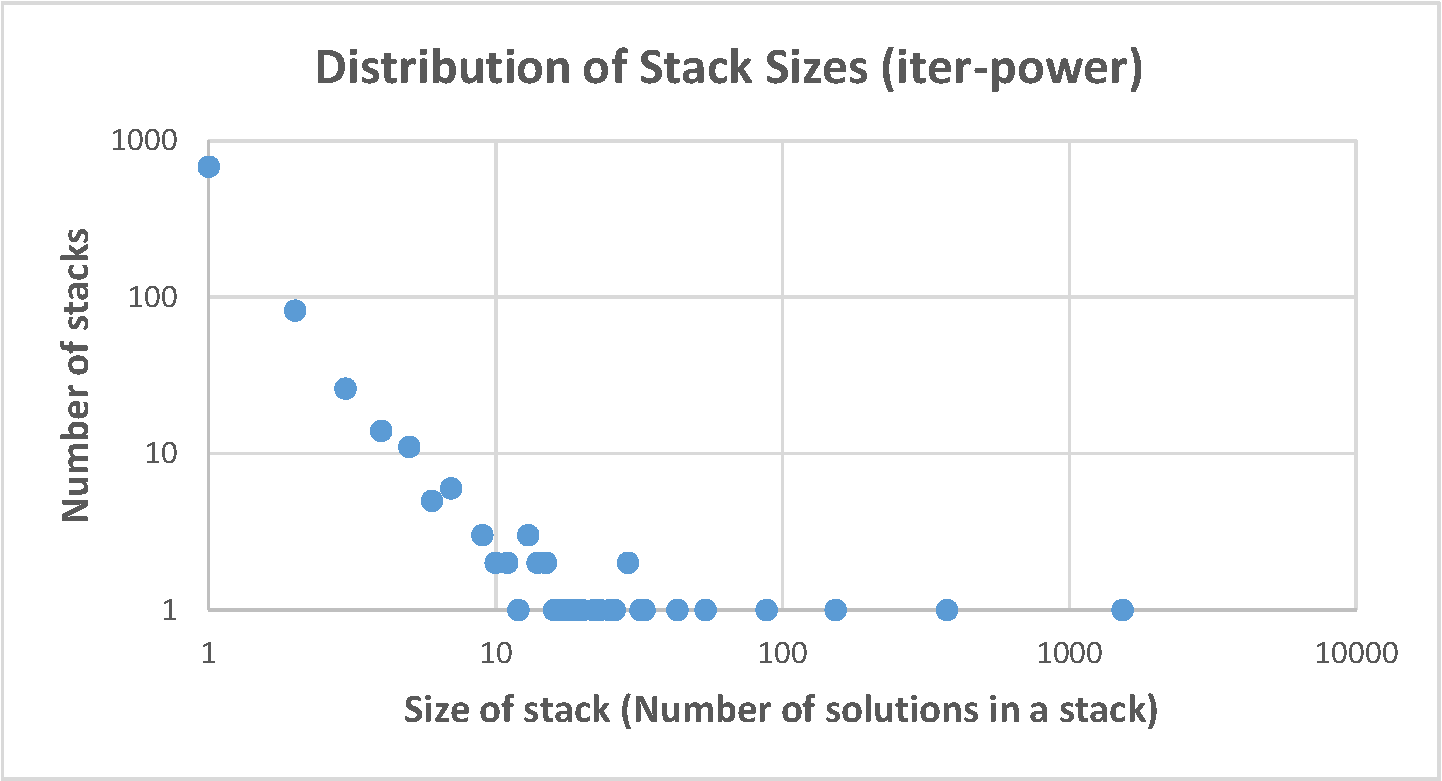
\includegraphics[scale=0.30]{Body/figures/overcode/stacksdistr-iter-power}
&
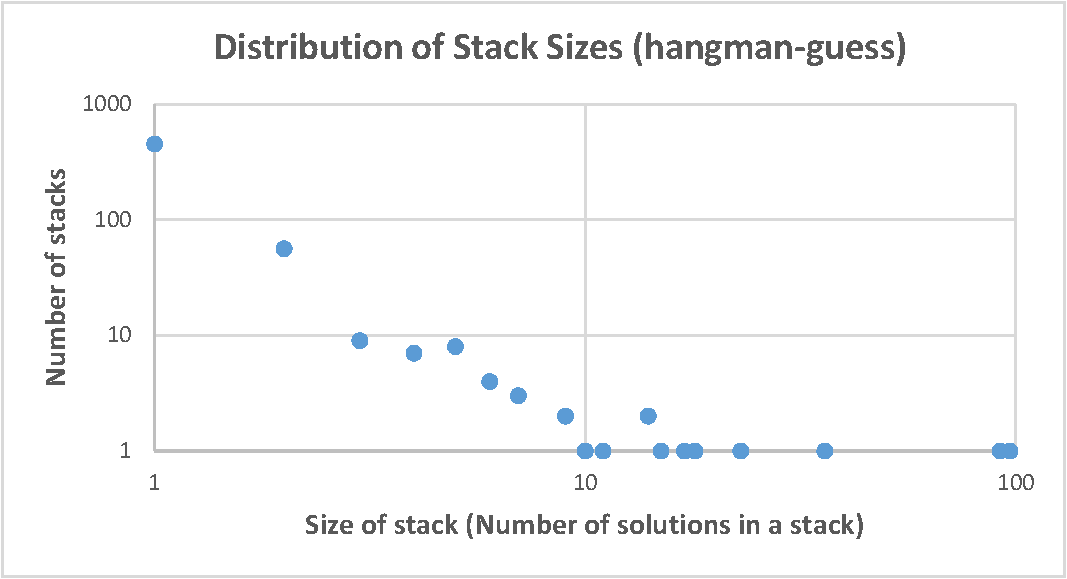
\includegraphics[scale=0.405]{Body/figures/overcode/stacksdistr-hangman}
\end{tabular}
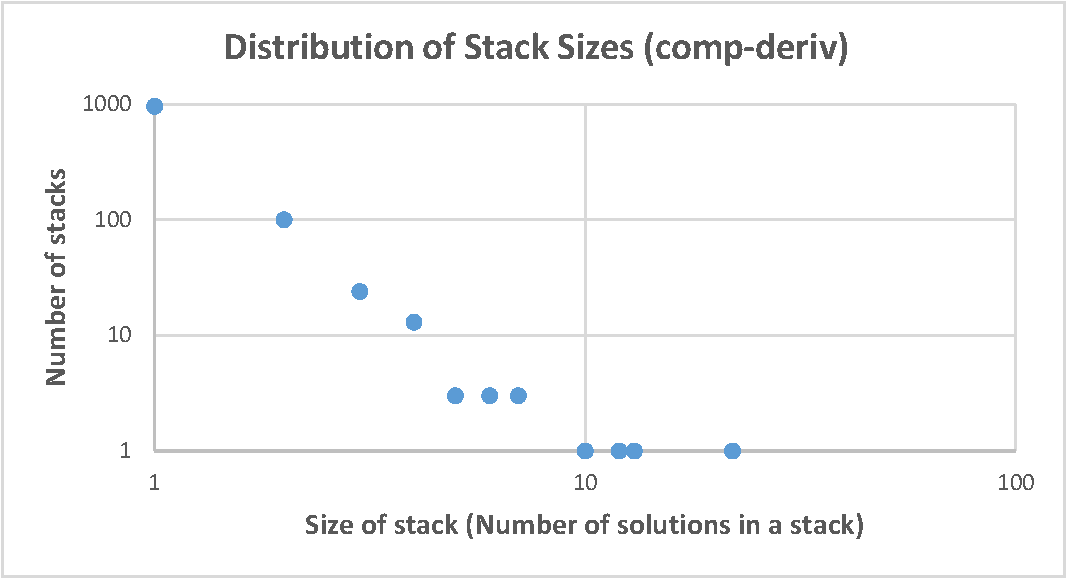
\includegraphics[scale=0.38]{Body/figures/overcode/stacksdistr-comp-deriv}
\caption{The distribution of sizes of the initial stacks generated by our algorithm for each problem, showing a long tail distribution with a few large stacks and a lot of small stacks. Note that the two axes corresponding to the size of stacks and the number of stacks are in logarithmic scale.}
\label{stackdistribution}
\end{figure*}

\begin{figure}[h!]
\begin{tabular}{c}
\\
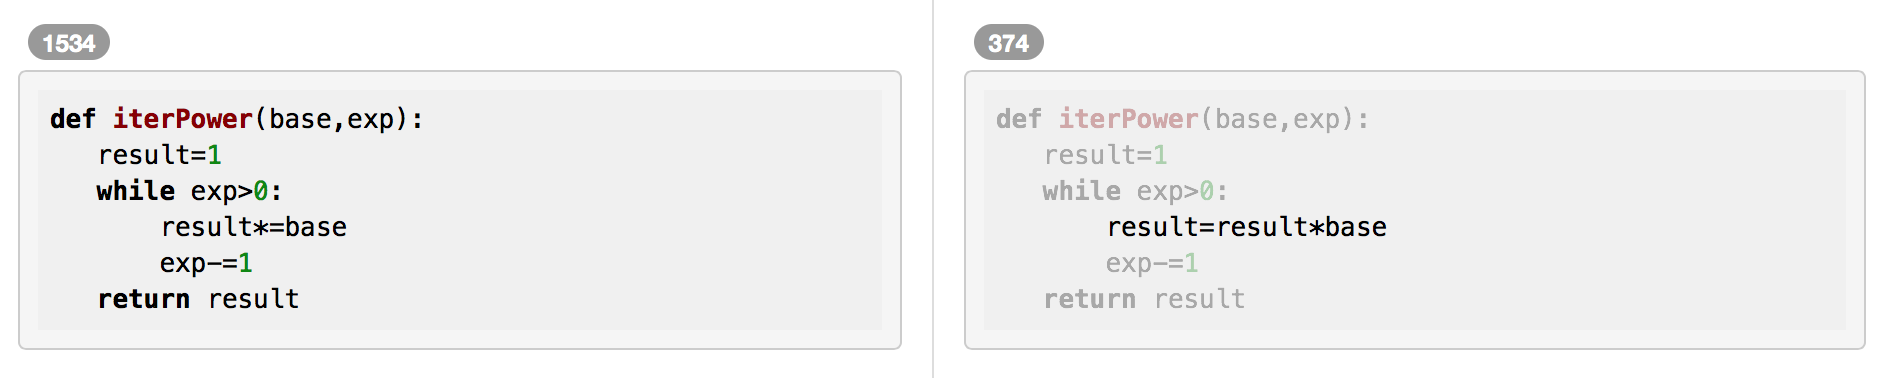
\includegraphics[scale=0.42]{Body/figures/overcode/iterpower-toptwo}
\\ (a) \\ \\
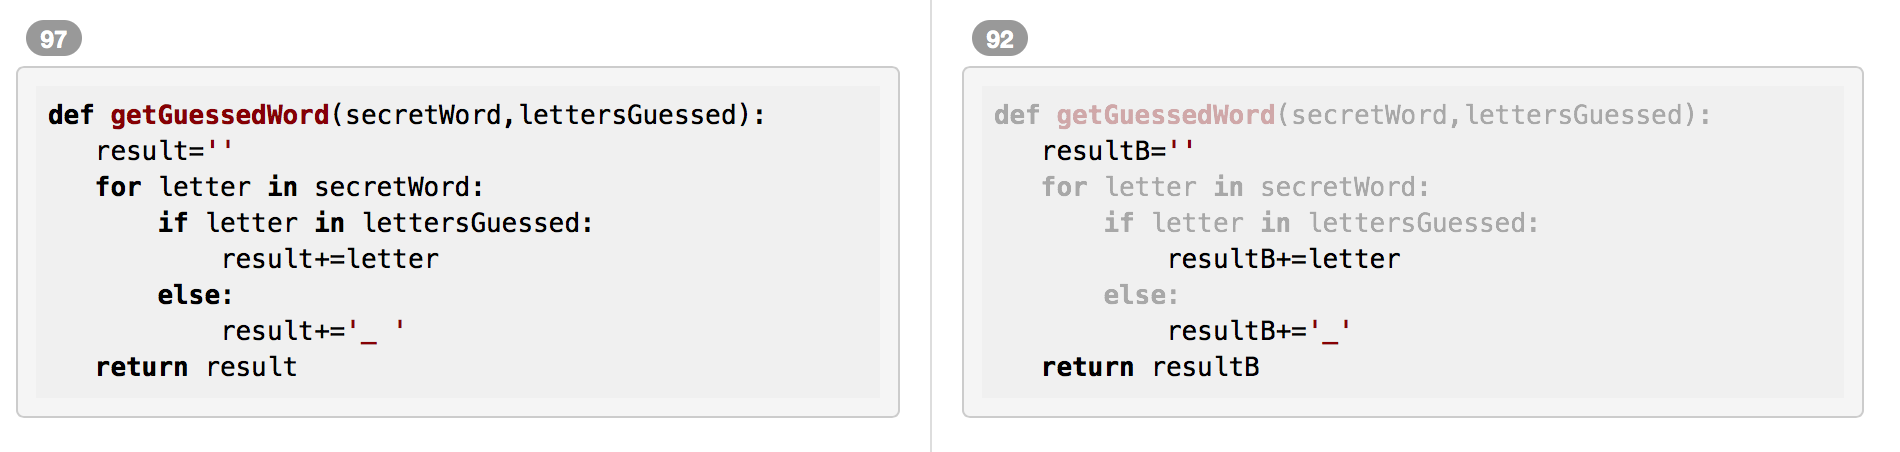
\includegraphics[scale=0.42]{Body/figures/overcode/hangman-toptwo}
\\ (b) \\ \\
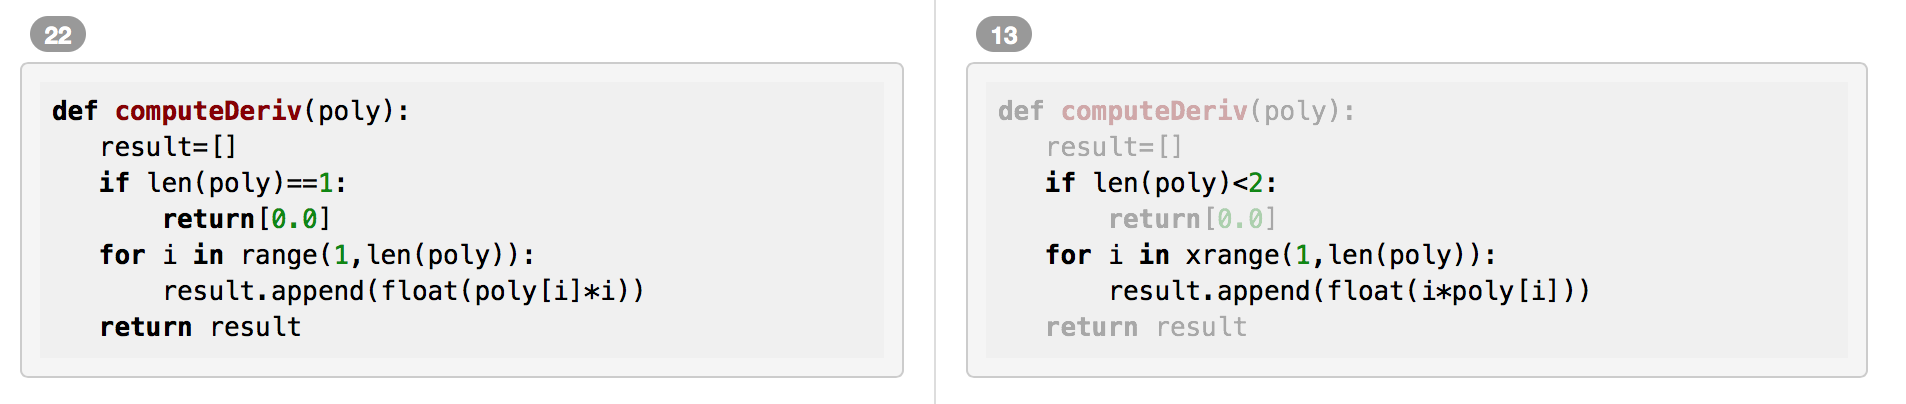
\includegraphics[scale=0.42]{Body/figures/overcode/compderiv-toptwo}
\\ (c) \\
\end{tabular}
\caption{The two largest stacks generated by the OverCode backend algorithm for the (a) \codevar{iterPower}, (b) \codevar{hangman}, and (c)  \codevar{compDeriv} problems.}
\label{toptwostacks}
\end{figure}

{\bf Common Variables} There exists a large variation among the variable names used by students to denote variables that compute the same set of values. The Variable Renaming step of the analysis renames these equivalent variables with the most frequently chosen variable name so that a teacher can easily recognize the role of variables in a given solution. The number of common variables found by the pipeline on the dataset problems is shown in Figure~\ref{backendevaluation} and some examples of these common variable names are shown in Figure~\ref{examplecommonvars}. Figure~\ref{examplecommonvars} also presents the number of times such a variable occurs across the solutions of a given problem, the corresponding variable sequence value on a given test input, and a subset of the original variable names used in the student solutions. 

\begin{figure}
\centering
\scriptsize
\begin{tabular} {|l|r|c|l|}
\hline
{\bf Common} & {\bf Occur} &  \multirow{3}{*}{\bf Sequence of Values} & \multirow{3}{*}{\bf Original Variable Names} \\
{\bf Variable} & {\bf -rence} & & \\
{\bf Name} & {\bf Count} & & \\
 \hline \hline
\multicolumn{4}{|c|}{}\\
\multicolumn{4}{|c|}{\bf iterPower}\\\hline
\codevar{result} & 3081 & [1,5.0,25.0,125.0] & \codevar{result}, \codevar{wynik}, \codevar{out}, \codevar{total}, \codevar{ans}, \codevar{acum}, \codevar{num}, \codevar{mult}, \codevar{output}, $\cdots$\\ \hline
\codevar{exp} & 2744 & [3,2,1,0] & \codevar{exp}, \codevar{iterator}, \codevar{app}, \codevar{ii}, \codevar{num}, \codevar{iterations}, \codevar{times}, \codevar{ctr}, \codevar{b}, $\cdots$\\ \hline
\codevar{exp} & 749 & [3] & \codevar{exp}, \codevar{count}, \codevar{temp}, \codevar{exp3}, \codevar{exp2}, \codevar{exp1}, \codevar{inexp}, \codevar{old\_exp}, $\cdots$\\ \hline
\codevar{i} & 266 & [0,1,2] & \codevar{i}, \codevar{a}, \codevar{count}, \codevar{c}, \codevar{b}, \codevar{iterValue}, \codevar{iter}, \codevar{n}, \codevar{y}, \codevar{inc}, \codevar{x},\codevar{times}, $\cdots$\\ \hline
\multicolumn{4}{|c|}{}\\
\multicolumn{4}{|c|}{\bf hangman}\\\hline
\codevar{letter} & 817 &  [`t',`i',`g',`e',`r'] & \codevar{letter}, \codevar{char}, \codevar{item}, \codevar{i}, \codevar{letS}, \codevar{ch}, \codevar{c}, \codevar{lett}, $\cdots$\\ \hline
\codevar{result} & 291 & [` ',`\_',`\_i',`\_i\_',`\_i\_e',`\_i\_e\_'] & \codevar{result}, \codevar{guessedWord}, \codevar{ans}, \codevar{str1}, \codevar{anss}, \codevar{guessed}, \codevar{string}, $\cdots$\\ \hline
\codevar{i} & 185 & [0,1,2,3,4] & \codevar{i}, \codevar{x}, \codevar{each}, \codevar{b}, \codevar{n}, \codevar{counter}, \codevar{idx}, \codevar{pos} $\cdots$\\ \hline
\codevar{found} & 76 & [0,1,0,1,0] & \codevar{found}, \codevar{n}, \codevar{letterGuessed}, \codevar{contains}, \codevar{k}, \codevar{checker}, \codevar{test}, $\cdots$\\ \hline
\multicolumn{4}{|c|}{}\\
\multicolumn{4}{|c|}{\bf compDeriv}\\ \hline
\codevar{result} & 1186 & [[],[0.0],$\cdots$,[0.0,35.0,9.0,4.0]] & \codevar{result}, \codevar{output}, \codevar{poly\_deriv}, \codevar{res}, \codevar{deriv}, \codevar{resultPoly}, $\cdots$\\ \hline
\codevar{i} & 284 &  [-13.39,0.0,17.5,3.0,1.0] & \codevar{i}, \codevar{each}, \codevar{a}, \codevar{elem}, \codevar{number}, \codevar{value}, \codevar{num}, $\cdots$\\ \hline
\codevar{i} & 261 & [0,1,2,3,4,5] & \codevar{i}, \codevar{power}, \codevar{index}, \codevar{cm}, \codevar{x}, \codevar{count}, \codevar{pwr}, \codevar{counter}, $\cdots$\\ \hline
\codevar{length} & 104 & [5] & \codevar{length}, \codevar{nmax}, \codevar{polyLen}, \codevar{lpoly}, \codevar{lenpoly}, \codevar{z}, \codevar{l}, \codevar{n}, $\cdots$\\ \hline

\end{tabular}
\caption{Some examples of common variables found by our analysis across the problems in the dataset. The table also shows the frequency of occurrence of these variables, the common sequence of values of these variables on a given test case, and a subset of the original variable names used by students.}
\label{examplecommonvars}
\end{figure}

{\bf Collisions in Variable Renaming} The number of Common/Common, Multiple Instances, and Unique/Common collisions discovered and resolved while performing variable renaming is shown in Figure~\ref{collisions}. A large majority of the collisions were Common/Common Collisions. For example, Figure~\ref{examplecommonvars} shows the common variable name \codevar{exp} for two different sequences of values $[3,2,1,0]$ and $[3]$ for the \codevar{iterPower} problem. Similarly, the common variable name \codevar{i} corresponds to sequences $[-13.9, 0.0, 17.5, 3.0, 1.0$ and $[0, 1, 2, 3, 4, 5]$ for the \codevar{compDeriv} problem. There were also a few Multiple Instances collisions and Unique/Common collisions found: 1.5\% for \codevar{iterPower}, 3\% for \codevar{compDeriv}, and 10\% for \codevar{hangman}.

\begin{figure}[htpb]
\centering
\begin{tabular}{|l|r|r|r|r|}
\hline
\multirow{2}{*}{\bf Problem} & {\bf Correct} & {\bf Common/Common} & {\bf Multiple Instances} & {\bf Unique/Common}\\
& {\bf Solutions} & {\bf Collisions } & {\bf Collisions} & {\bf Collisions}\\
\hline \hline
\codevar{iterPower} & 3875 & 1298 & 25 & 32 \\ \hline
\codevar{hangman} & 1118 & 672 & 62 & 49\\ \hline
\codevar{compDeriv} & 1433 & 928 & 21 & 23 \\ \hline
\end{tabular}
\caption{The number of common/common, multiple instances, and unique/common collisions discovered by our algorithm while renaming the variables to common names.}
\label{collisions}
\end{figure}

\section{User Studies}

The goal was to design a system that allows teachers to develop a better understanding of the variation in student solutions, and give feedback that is relevant to more student solutions. Two user studies were designed to evaluate our progress in two ways: (1) user interface satisfaction and (2) how many solutions teachers could read and produce feedback on in a fixed amount of time. Reading and providing feedback to thousands of solutions is an unrealistically difficult task for the control condition, so instead of measuring time to finish the entire set of solutions, the experiment measures what subjects could accomplish in a fixed amount of time (15 minutes).

Together, these studies test four hypotheses:
\begin{itemize}
\item \textbf{H1 Interface Satisfaction} Subjects will find OverCode easier to use, more helpful and less overwhelming for browsing thousands of solutions, compared to the baseline. 

\item {\bf H2 Read coverage and speed} Subjects are able to read code that represents more student solutions at a higher rate using OverCode than with the baseline. 

\item {\bf H3 Feedback coverage} Feedback produced when using OverCode is relevant to more student solutions than when feedback is produced using the baseline.

\item {\bf H4 Perceived coverage} Subjects feel that they develop a better high-level view of students' understanding and misconceptions, and provide more relevant feedback using OverCode than with the baseline.

\end{itemize}

\subsection{User Study 1: Writing a Class Forum Post}

The first study was a 12-person within-subjects evaluation of interface satisfaction when using OverCode for a realistic, relatively unstructured task. Using either OverCode or a baseline interface, subjects were asked to browse student solutions to the programming problems in our dataset and then write a class forum post on the good and bad ways students solved the problem. Through this study, the first hypothesis is tested.

\subsubsection{OverCode and Baseline Interfaces}

Two interfaces were designed, referred to here as OverCode and the baseline. The OverCode interface and backend are described in detail in Section \ref{overcode}. The baseline interface was a single webpage with all student solutions concatenated in a random order into a flat list (Figure \ref{iterPowerEdXControl}, left). This design emulates existing methods of reviewing solutions, and aims to draw out differences between browsing stacked and unstacked solutions. This is analogous to the ``flat'' interface chosen as a baseline for Basu et al.'s interface for grading clusters of short answers~\cite{basuDivideAndConquer}. Basu et al.'s assumption, that existing options for reviewing solutions are limited to going through solutions one-by-one, is backed by our pilot studies and interviews with teaching staff, and our own grading experiences. In fact, in edX programming MOOCs, teachers are not even provided with an interface for viewing all solutions at once. They can only look at one student solution at a time. If the solutions can be downloaded locally, some teachers may use a search tool like \codevar{grep}. Our baseline allows for search too, through the in-browser \texttt{Find} command. 

In the baseline, solutions appeared visually similar to those in the OverCode interface (boxed, syntax-highlighted code), but the solutions were raw, in the sense that they were not normalized for whitespace or variable naming differences. As in the OverCode condition, subjects were able to use standard web-browser features, such as the within-page \texttt{Find} action.


\begin{figure}[h!]
\centering
\begin{tabular}{cc}
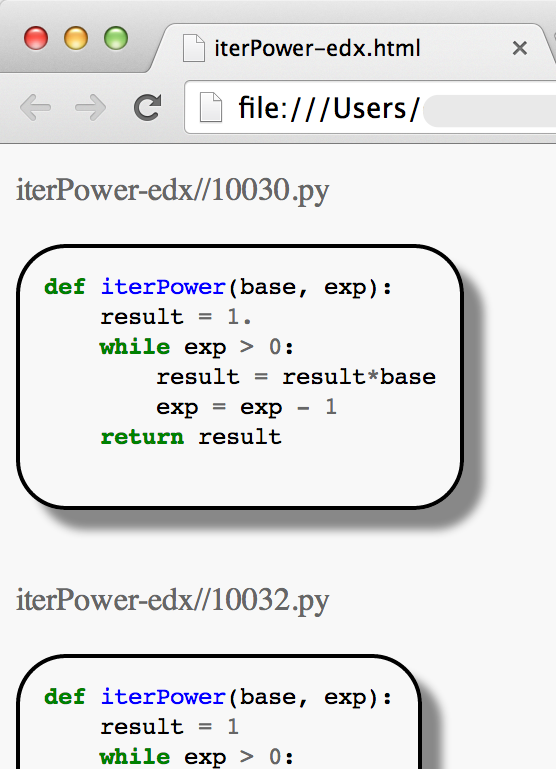
\includegraphics[scale=0.5]{Body/figures/overcode/iterPowerEdXControlStudy1.png} &
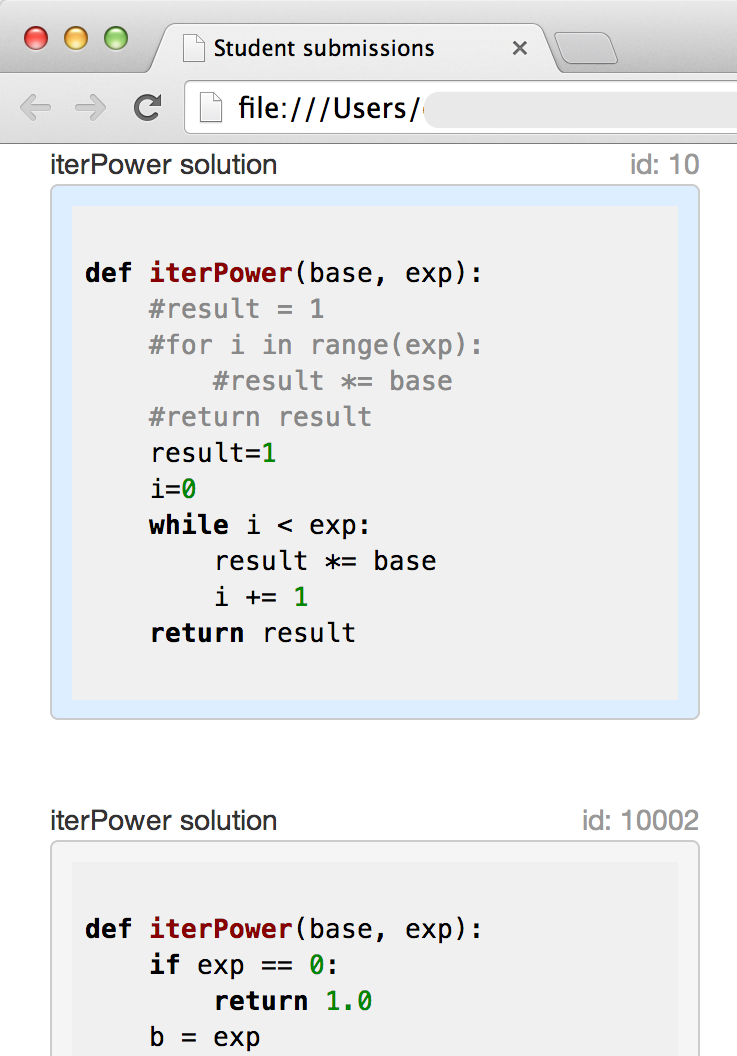
\includegraphics[scale=0.37]{Body/figures/overcode/iterPowerEdXControlStudy2.png} \\
\end{tabular}
\caption{Screenshots of the baseline interface. The appearance did not change significantly between the Forum Post study control interface, shown on the left, and the Coverage study control interface, shown on the right. Functionality did not change at all.}
\label{iterPowerEdXControl}
\end{figure}

\subsubsection{Participants}

Participants were recruited by reaching out to past and present programming course staff at our university, and advertising on an MIT CSAIL email list. These individuals were qualified to participate in our study because they met at least one of the following requirements: (1) have taught a computer science course (2) have graded Python code before, or (3) have significant Python programming experience, making them potential future teaching staff. Subjects were offered \$20 to participate. 

Information about the subjects' backgrounds was collected during recruitment and again at the beginning of their one-hour in-lab user study session. 12 people (7 male) participated, with a mean age of 23.5 ($\sigma = 3.8$). Subjects had a mean 4 years of Python programming experience ($\sigma = 1.8$), and $75\%$ of participants had graded student solutions written in Python before. Half of the participants were graduate students and the other half were undergraduates.

\subsubsection{Apparatus}

Subjects used laptops running MacOS and Linux with screen sizes ranging from 12.5 to 15.6 inches, and viewed the OverCode and baseline interfaces in either Safari or Chrome. Data was recorded with Google Docs and Google Forms filled out by participants.

\subsubsection{Conditions}

Subjects performed the main task of browsing solutions and writing a class forum post twice, once in each interface condition, focusing on one of the three problems in our dataset (Section \ref{dataset}) each time. For each participant, the third remaining problem was used during training, to reduce learning effects when performing the two main tasks. The pairing and ordering of interface and problem conditions were fully counterbalanced, resulting in 12 total conditions. The twelve participants were randomly assigned to one of the 12 conditions, such that all conditions were tested.

\subsubsection{Procedure}

{\bf Prompt} The experimenter began by reading the following prompt, to give the participant context for the tasks they would be performing:

\begin{quote}

We want to help TAs [teaching assistants] give feedback to students in programming classes at scale. For each of three problems, we have a large set of students' submissions ($> 1000$). 

All the submissions are correct, in terms of input and output behavior. We're going to ask you to browse the submissions and produce feedback for students in the class. You'll do this primarily in the form of a class forum post.
\end{quote}

To make the task more concrete, participants were given an example\footnote{Our example was drawn from the blog ``Practice Python: 30-minute weekly Python exercises for beginners,'' posted on Thursday, April 24, 2014, and titled ``SOLUTION Exercise 11: Check Primality and Functions.'' (\url{http://practicepython.blogspot.com})} of a class forum post that used examples taken from student solutions to explain different strategies for solving a Python problem. They were also given print-outs of the prompts for each of the three problems in our dataset, to reference when looking at solutions.

{\bf Training} Given the subjects' extensive experience with web-browsers, training for the baseline interface was minimal. Prior to using the OverCode interface, subjects watched a 3-4 minute long training video demonstrating the features of OverCode, and were given an opportunity to become familiar with the interface and ask questions. The training session focused on the problem that would not be used in the main tasks, in order to avoid learning effects.

{\bf Tasks} Subjects then performed the main tasks twice, once in each interface, focusing on a different programming problem each time. They were given a fixed amount of time to both read solutions and provide feedback, so task completion times were not measured, but instead the quality of their experience in providing feedback to students at scale.

\begin{itemize}
\item {\it Feedback for Students} (15 minutes) Subjects were asked to write a class forum post on the good and bad ways students solved the problem. The 15-minute period included both browsing and writing time, as subjects were free to paste in code examples and write comments as they browsed the solutions.

\item {\it Autograder Bugs} (2 min) Although the datasets of student solutions were marked as correct by an autograder, there may be holes in the autograder test cases. Some solutions may deviate from the problem prompt, and therefore be considered incorrect by teachers, e.g., recursive solutions to \codevar{iterPower} when its prompt explicitly calls for an iterative solution. As a secondary task, subjects were asked to write down any bugs in the autograder they came across while browsing solutions. This was often performed concurrently with the primary task by the subject.
\end{itemize}
{\bf Surveys} Subjects filled out a post-interface condition survey about their experience using the interface. This was a short-answer survey, where they wrote about what they liked, what they did not like, and what they would like to see in a future version of the interface. At the end of the study, subjects rated agreement (on a 7-point Likert scale) with statements about their satisfaction with each interface.

\subsubsection{Results}
Figure~\ref{study1Likert} shows that, compared to the control interface, subjects find OverCode less overwhelming, easier to use, and more helpful for getting a sense of students' understanding. After using both interfaces to view thousands of solutions, subjects found OverCode easier to use ($W=52, Z=2.41, p<0.05, r=0.70$) and less overwhelming ($W=0, Z=-2.86, p<0.005, r=0.83$) than the baseline interface. Finally, participants felt that OverCode ``helped me get a better sense of my students' understanding'' than the baseline did ($W=66, Z=3.04, p<0.001, r=0.88$). These differences are statistically significant, as computed by the Wilcoxon Signed Rank test with pairing users' ratings of each interface. This supports \textbf{H1}.

\begin{figure}
\centering
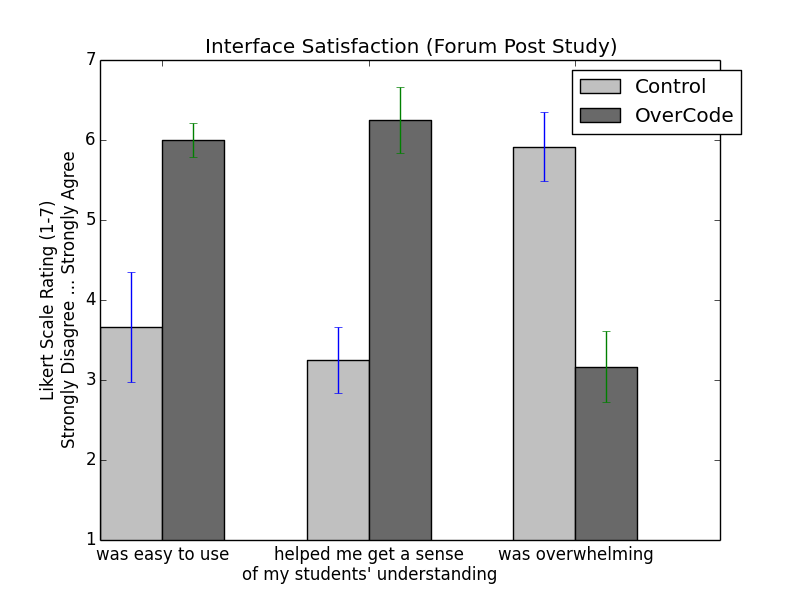
\includegraphics[scale=0.5]{Body/figures/overcode/study1Likert.png}
\caption{{\bf H1: Interface satisfaction} Mean Likert scale ratings (with standard error) for OverCode and baseline interfaces, after subjects used both to perform the forum post writing task.}
\label{study1Likert}
\end{figure}


From the surveys conducted after subjects completed each interface condition, subjects found stacking and the ability to rewrite code to be useful and enjoyable features of OverCode:
\begin{itemize}
\item {\it Stacking is an awesome feature. Rewrite tool is fantastic. Done feature is very rewarding--feels much less overwhelming. "Lines that appear in x submissions" also awesome.}

\item {\it Really liked the clever approach for variable normalization. Also liked the fact that stacks showed numbers, so I'd know I'm focusing on the highest-impact submissions. Impressed by the rewrite ability... it cut down on work so much!}

\item {\it I liked having solutions collapsed (not having to deal with variable names, etc), and having rules to allow me to collapse even further. This made it easy to see the ``plurality'' of solutions right away; I spent most of the time looking at the solutions that only had a few instances.}
\end{itemize}

When asked for suggestions, participants gave many suggestions on stacks, filtering, and rewrite rules, such as:
\begin{itemize}
\item Enable the teacher to change the main stack that is being compared against the others.
\item Suggest possible rewrite rules, based on what the teacher has already written, and will not affect the answers on the test case.
\item Create a filter that shows all stacks that do {\it not} have a particular statement.
\end{itemize}

For both the OverCode and baseline interfaces, the feedback generated about \codevar{iterPower}, \codevar{hangman}, and \codevar{compDeriv} solutions fell into several common themes. One kind of feedback suggested new language features, such as using \codevar{*=} or the keyword \codevar{in}. Another theme identified inefficient, redundant, and convoluted control flow, such as repeated statements and unnecessary statements and variables. It was not always clear what the misconception was, though, as one participant wrote, \textit{``The double iterator solution surely shows some lack of grasp of power of for loop, or range, or something.''} Participant feedback included comments on the relative goodness of different correct solutions in the dataset. This was a more holistic look at student solutions as they varied along the dimensions of conciseness, clarity, and efficiency previously described.

Study participants found both noteworthy correct solutions and solutions they considered incorrect, despite passing the autograder. One participant learned a new Python function, \codevar{enumerate}, while looking at a solution that used it. The participant wrote, \textit{``Cool, but uncalled for. I had to look it up :]. Use, but with comment.''} Participants also found recursive \codevar{iterPower} and \codevar{hangman} solutions, which they found noteworthy. For what should have been an iterative \codevar{iterPower} function, the fact that this recursive solution was considered correct by the autograder was considered an autograder bug by some participants. Using the built-in Python exponentiation operator \codevar{**} was also considered correct by the autograder, even though it subverted the point of the assignment. It was also noted as an autograder bug by some participants who found it.

\subsection{User Study 2: Coverage}

A second 12-person study was designed, similar in structure to the forum post study, but focused on measuring the coverage achieved by subjects in a fixed amount of time (15 minutes) when browsing and producing feedback on a large number of student solutions. The second study's task was more constrained than the first: instead of writing a freeform post, subjects were asked to identify the five most frequent strategies used by students and rate their confidence that these strategies were frequently used in the student solutions. These changes to the task enabled us to measure coverage in terms of solutions read, the relevance of written feedback and the subject's perceived coverage. In this study, the rest of the hypotheses, i.e., H2, H3, and H4, are tested.

Prior to running the second study, both the OverCode and baseline interfaces were slightly modified. Figure \ref{iterPowerEdXControl} shows the baseline changes that reduce the differences between the rendering of solutions in the baseline and OverCode interfaces. The OverCode interface was changed to show identifiers next to every stack and solutions so that subjects could provide it when asked.

\subsubsection{Participants, Apparatus, Conditions}

The coverage study shared the same methods for recruiting participants, apparatus and conditions as the forum post study. 12 new participants (11 male) participated in the second study (mean age = 25.4, $\sigma = 6.9$). Across those 12 participants, the mean years of Python programming experience was 4.9 ($\sigma = 3.0$) and 9 of them had previously graded code (5 had graded Python code). There were 5 graduate students, 6 undergraduates, and 1 independent computer software professional.


\subsubsection{Procedure}
{\bf Prompt} In the coverage study, the prompt was similar to the one used in the forum post study, explaining that the subjects would be tackling the problem of producing feedback for students at scale. The language was modified to shift the focus towards finding frequent strategies used by students, rather than any example of good or bad code used by a student.\todo{find prompt and put it in here}

{\bf Training} As before, subjects were shown a training video and given time to practice using OverCode features prior to their trial in the OverCode condition.

{\bf Task} The coverage study task consisted of a more constrained feedback task. Given 15 minutes with either the OverCode or baseline interface, subjects were asked to fill out a table, identifying the five most frequent strategies used by students to solve the problem. For each strategy they identified, they were asked to fill in the following fields in the table:
\begin{itemize}
\item A code example taken from the solution or stack.
\item The identifier of the solution or stack.
\item A short (one sentence) annotation of what was good or bad about the strategy.
\item Their confidence, on a scale of 1-7, that the strategy frequently occurred in the student solutions.
\end{itemize}
Importantly, subjects were also asked to mark solutions or stacks as \emph{read} by clicking on them after they had processed them, even if they were not choosing them as representative strategies. Combined with interaction logging done by the system, this enabled us to measure read coverage.

{\bf Surveys} Although we measured interface satisfaction for a realistic task in the forum post study, we also measured interface satisfaction through surveys for this more constrained, coverage-focused task. Subjects filled out a post-interface condition survey in which they rated agreement (on a 7-point Likert scale) with positive and negative adjectives about their experience using the interface, and reflected on task difficulty. At the end of the study, subjects were asked to rate their agreement with statements about the usefulness of specific features of both the OverCode and baseline interfaces, and responded to the same interface satisfaction 7-point Likert scale statements used in the first study.

\subsubsection{Results} \label{coverageResults}
\begin{figure*}[b!]
\begin{tabular}{c | c}
\begin{minipage}{.5\linewidth}
\centering
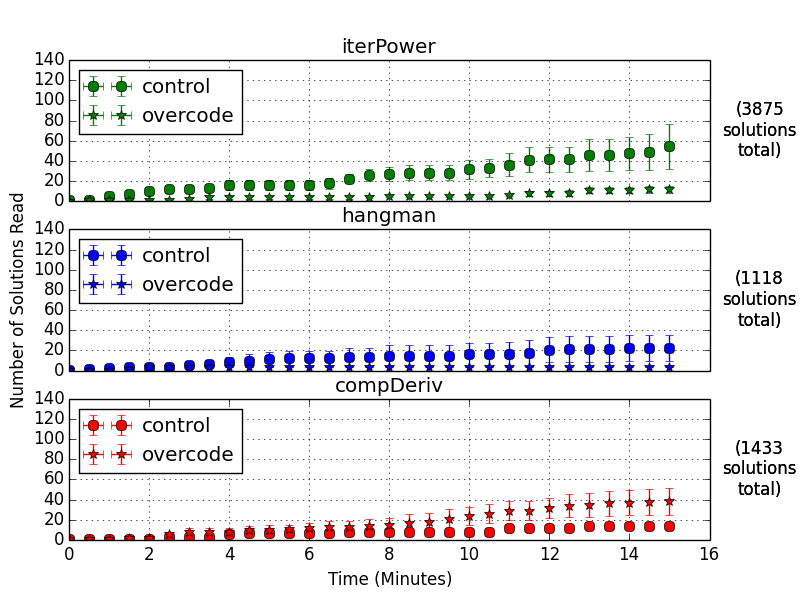
\includegraphics[width=\linewidth]{Body/figures/overcode/prettyReadCoverage.png}
\end{minipage}
&
\begin{minipage}{.5\linewidth}
\centering
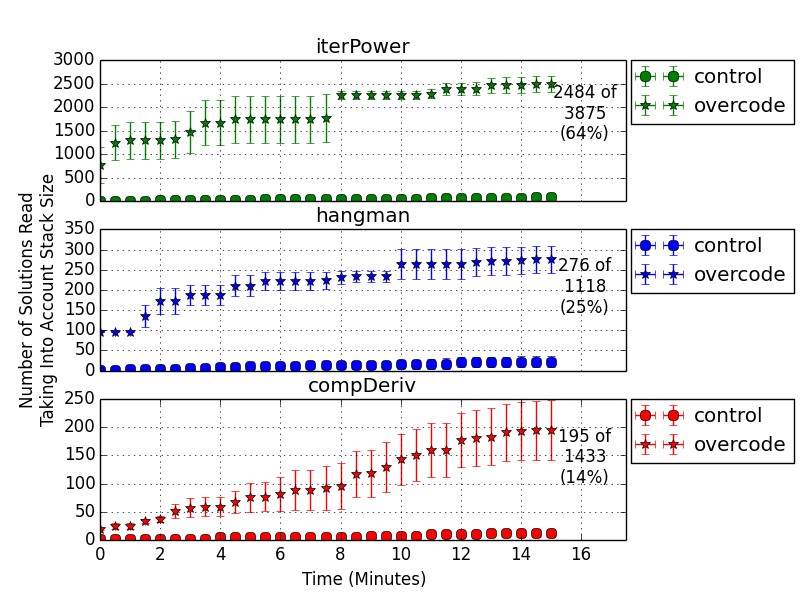
\includegraphics[width=\linewidth]{Body/figures/overcode/prettyPercentCoverage.png}
\end{minipage}
\\
(a) & (b)
\end{tabular}
\caption{In (a), we plot the mean number of platonic solutions read in OverCode over time versus the number of raw solutions read in the baseline interface over time while performing the 15-minute Coverage Study task. In (b), we replace the mean number of platonic solutions with the mean number of solutions, i.e., the stack size, they represent. These are shown for each of the three problems in the dataset.}
\label{readCoverage}
\end{figure*}

{\bf H2: Read coverage and speed} Figure \ref{readCoverage} shows that subjects reading platonic \texttt{iterPower}, \texttt{hangman}, and \texttt{compDeriv} solutions in the OverCode interface covered the equivalent of 64\%, 25\%, and 14\% of all student solutions to those problems (Mann--Whitney U = 16, n1 = n2 = 4, p<0.05). Subjects read through more raw solutions than platonic solutions to the simplest problems, i.e., \texttt{iterPower} and \texttt{hangman}, but when problem difficulty increased, i.e., \texttt{compDeriv}, subjects read through OverCode's platonic solutions faster than raw solutions. This supports the H2 hypothesis.

%This hypothesis is supported by our measurements of read coverage from this study. For each problem, subjects were able to view more normalized and stacked solutions by the end of the 15-minute-long main task using OverCode than raw solutions when using the baseline interface (Mann--Whitney U = 16, n1 = n2 = 4, p<0.05). Figure \ref{readCoverage} shows the mean number of solutions read over time for each interface and each problem in our dataset. The curves show that subjects were able to read code that represented more raw solutions at a higher rate due to the stacking of similar solutions.

{\bf H3: Feedback coverage} Each subject reported on the five most frequent strategies in a set of solutions, by copying both a code example and the identifier of the solution (baseline) or stack (OverCode) that it came from. We define \emph{feedback coverage} as the number of students for which the quoted code is relevant, in the sense that they wrote the same lines of code, ignoring differences in whitespace or variable names. We computed the coverage for each example using the following process:
\begin{itemize}
\item Reduce the quoted code down to only the lines referred to in the annotation. Often, the subject's annotation would focus on a specific feature of the quoted code, which sometimes had additional lines that were unrelated to the subject's feedback. For example, comments about iterating over a range function, while also quoting the contents of the for loop. This step meant we would be calculating the coverage of a more general (smaller) set of lines.

\item Find the source stack that the quoted code comes from. This is trivial in the OverCode condition, where the stack ID is included in the subject's post. In the baseline, we used the solution ID included in the subject's post to find the stack that it was merged into by the backend pipeline.

\item Find the normalized version of each quoted line. The quoted lines of code may be raw code if they come from the baseline condition. By comparing the quoted code with the normalized code of its source stack, we found the normalized version of each line, with variable names and whitespace normalized.

\item Find the raw solutions that include the set of normalized lines, using a map from stacks to raw solutions provided by the backend pipeline.
\end{itemize}

\begin{figure}[b!]
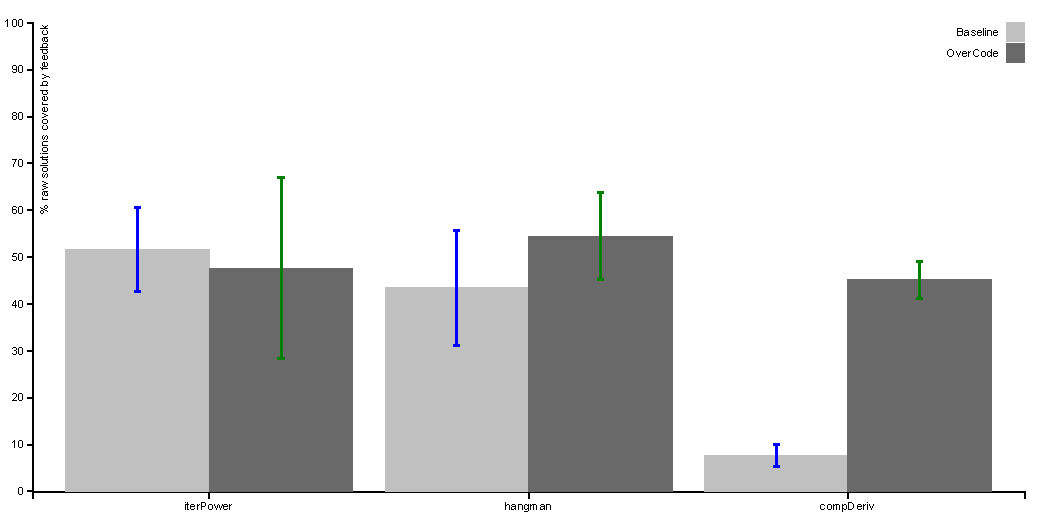
\includegraphics[width=0.6\paperwidth]{Body/figures/overcode/feedbackCoverage.pdf}
\caption{Mean feedback coverage, i.e., the percentage of raw solutions covered, per trial during the coverage study for each problem, in the OverCode and baseline interfaces.}
\label{aveCoveragePerPost}
\end{figure}
%\todo{DNHT: what are the error bars?}

Figure \ref{aveCoveragePerPost} shows the mean coverage of a set of feedback produced by a single subject, across problems and interface conditions. The feedback coverage is shown as the mean percentage of raw solutions for which the feedback was relevant. When giving feedback on the \codevar{iterPower} and \codevar{hangman} problems, there was not a statistically significant difference in the feedback coverage between interface conditions. However, on \codevar{compDeriv}, the problem with the most complex solutions, subjects using OverCode were able to achieve significantly more coverage of student solutions than when using the baseline interface (Mann--Whitney U = 0, n1 = n2 = 4, p< 0.05).

\begin{figure*}[t!]
\begin{tabular}{c | c}
\begin{minipage}{.5\linewidth}
\centering
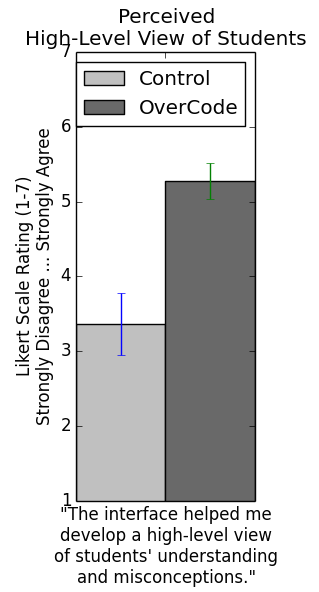
\includegraphics[scale=0.5]{Body/figures/overcode/highLevelViewStudy2.png}
\end{minipage}
&
\begin{minipage}{.5\linewidth}
\centering
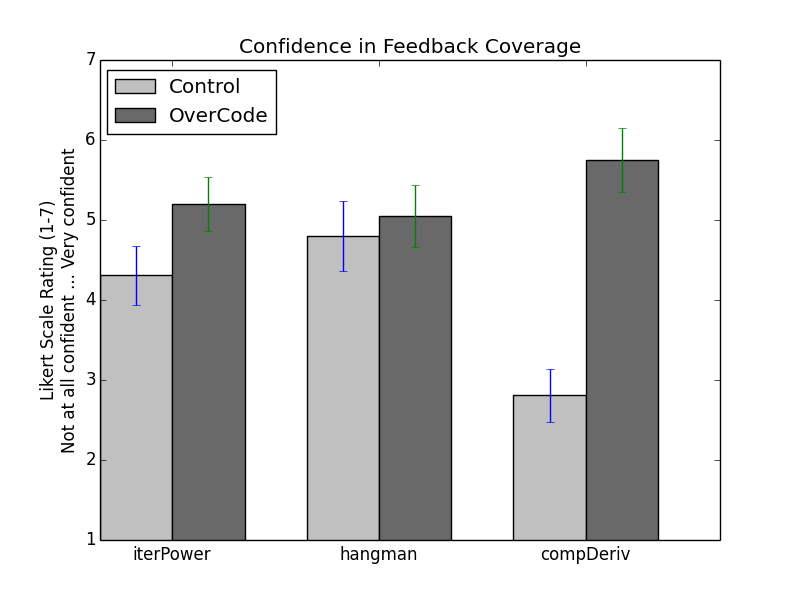
\includegraphics[width=\linewidth]{Body/figures/overcode/coverageConfidence.png}
\end{minipage}
\\
(a) & (b)
\end{tabular}
\caption{Mean rating with standard error for (a) post-condition perception of coverage (excluding one participant) and (b) confidence ratings that identified strategies were frequently used (1-7 scale).}
\label{perceivedCoverage}
\end{figure*}

{\bf H4: Perceived coverage} After using each interface, we asked participants how strongly they agreed with the statement `This interface helped me develop a high-level view of students' understanding and misconceptions,' which quotes the first part of our third hypothesis. Participants agreed with this statement after using OverCode significantly more than when using the baseline interface ($W=63, Z=2.70, p<0.01, r=0.81$). Statistical significance was computed using the Wilcoxon Signed Rank test, pairing users' ratings of each interface. The analysis was done on 11 participants' data, as one participant's data was lost. The mean rating with standard error for the responses is shown in Figure~\ref{perceivedCoverage}(a). 

For each strategy identified by subjects, we asked them to rate their confidence, on a scale of 1-7, that the strategy was frequently used by students in the dataset. Mean confidence ratings on a per-problem basis are shown in Figure \ref{perceivedCoverage}(b). We found that for \codevar{compDeriv}, subjects using OverCode were significantly more confident that their annotations were relevant to many students, compared to the baseline (Mann--Whitney $U=260.5, n_{1}=18, n_{2}=16, p<0.0001$).
 
{\bf H1: Interface satisfaction} Interface satisfaction was measured through multiple surveys, (1) immediately after using each interface and (2) after using both interfaces. Statistical significance was computed using the Wilcoxon Signed Rank test, pairing users' ratings of each interface. 

Immediately after finishing the assigned tasks with an interface, participants rated their agreement with statements about the appropriateness of various adjectives to describe the interface they just used, on a 7-point Likert scale. While participants found the baseline to be significantly more simple ($W=2.5, Z=-2.60, p<0.01, r=0.78$), they found OverCode to be significantly more flexible ($W=45, Z=2.84, p<0.005, r=0.86$), less tedious ($W=3.5, Z=-2.41, p<0.05, r=0.73$), more interesting ($W=66, Z=2.96, p<0.001, r=0.89$), and more enjoyable ($W=45, Z=2.83, p<0.005, r=0.85$). The analysis was done on 11 participants' data, as one participant's data was lost. The mean ratings (with standard error) for the responses are shown in Figure~\ref{studyLikert1_onPop2}. 

After the completion of the Coverage Study, participants were asked again to rate their agreement with statements about each interface on a 7-point Likert scale. After using both interfaces to view thousands of solutions, there were no significant differences between how overwhelming or easy to use each interface was. However, participants did feel that OverCode ``helped me get a sense of my students' understanding'' more than the baseline ($W=62.5, Z=-2.69, p<0.01, r=0.78$). The mean ratings (with standard error) for the responses are shown in Figure~\ref{studyLikert1_onPop2}.

\begin{figure}
\centering
\begin{tabular}{c c}
\begin{minipage}{.6\linewidth}
\centering
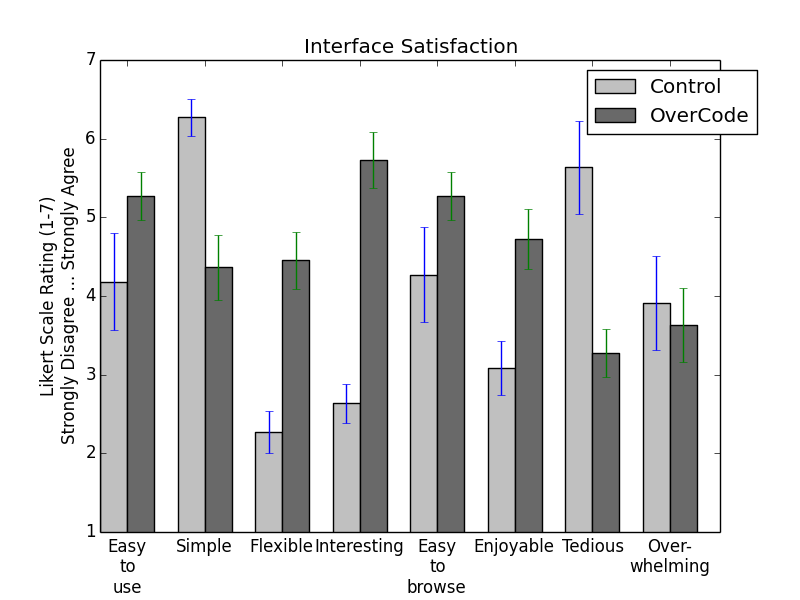
\includegraphics[scale=0.35]{Body/figures/overcode/study2Likert.png}
\end{minipage}
&
\begin{minipage}{.4\linewidth}
\centering
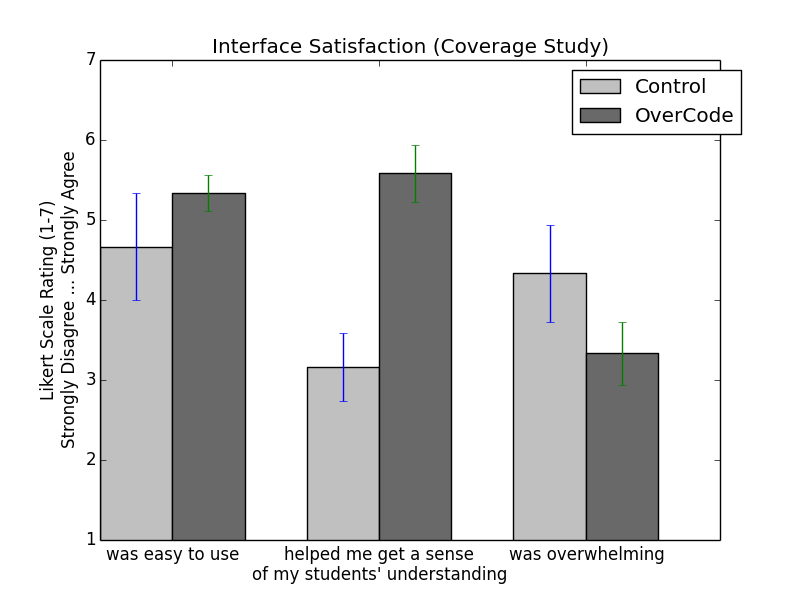
\includegraphics[scale=0.30]{Body/figures/overcode/study1Likert_onPop2.png}
\end{minipage}
\\
(a) & (b)
\end{tabular}
\caption{{\bf H1: Interface satisfaction} Mean Likert scale ratings (with standard error) for  OverCode and baseline, (a) immediately after using the interface for the Coverage Study task, and (b) after using both interfaces.}
\label{studyLikert1_onPop2}
\end{figure}

{\bf Usage and Usefulness of Interface Features} In the second part of the post-study survey, participants rated their agreement with statements about the helpfulness of various interface features on a 7-point Likert scale. There were only two features to ask about in the baseline interface (in-browser find and viewing raw solutions), which were mixed in with statements about features in the OverCode interface. The OverCode feature of stacking equivalent solutions was found more helpful than the baseline features of in-browser find ($W=41, Z=2.07, p<0.05, r=0.60$) and viewing raw student solutions, comments included ($W=45, Z=2.87, p<0.005, r=0.83$). The OverCode feature of variable renaming and previewing rewrite rules were also both found significantly more helpful than seeing raw student code ($W=65.5, Z=2.09, p<0.05, r=0.61$ and $W=56.5, Z=2.14, p<0.05, r=0.62$, respectively). The mean ratings for the features are shown in Figure~\ref{featureHelpfulness}.

\begin{figure}
\centering
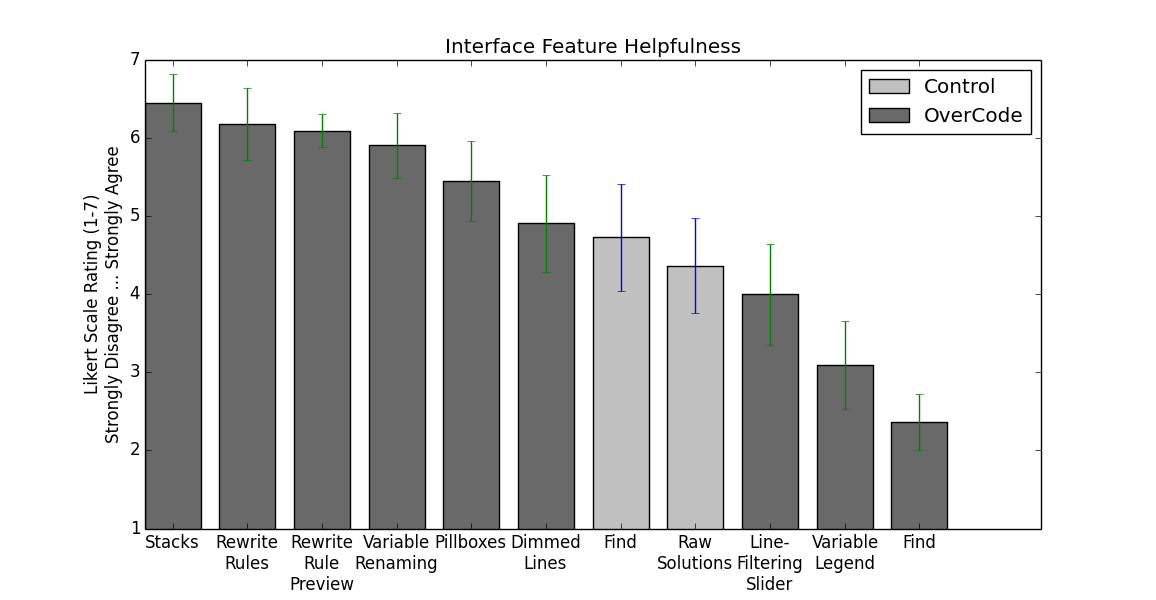
\includegraphics[scale=0.5]{Body/figures/overcode/featureHelpfulness.png}
\caption{Mean Likert scale ratings (with standard error) for the usefulness of features of OverCode and baseline. {\it Find} refers to the find function within the web browser. {\it Find} appears twice in this figure because users rated its usefulness for each condition.}
\label{featureHelpfulness}
\end{figure}

In addition to logging \codevar{read} events, we also recorded usage of interface features, such as creating rewrite rules and filtering stacks. A common usage strategy was to read through the stacks linearly and mark them as \codevar{read}, starting with the largest reference stack, then rewrite trivial variations in expressions to merge smaller behaviorally equivalent stacks into the largest stack. Stack filtering (Figure~\ref{linefilter}) was sometimes used to review solutions that contained a particularly conspicuous line, e.g., a recursive call to solve \codevar{iterPower} or an extremely long expression. The filter panel frequency slider (Figure~\ref{linefilter}a) and the variable legend (Figure~\ref{afterrewrite}b) were scarcely used.

All subjects wrote at least two rewrite rules, often causing stacks to merge that only differed in some trivial way, like reordering operands in multiplication statements, e.g., \codevar{result = result*base} vs. \codevar{result = base*result}. Some rewrite rules merged Python expressions that behaved similarly but differed in their verbosity, e.g., \codevar{for i in range(0, exp)} vs. \codevar{for i in range(exp)}. These variations may be considered noteworthy or trivial by different teachers.

\section{Discussion}

Our three-part evaluation of the OverCode backend and user interface demonstrates its usability and usefulness in a realistic teaching scenario. Given that we focused on the first three weeks of an introductory Python programming course, our evaluation is limited to single functions, whose most common solutions were less than ten lines long. Some of these functions were recursive, while most were iterative. Variables were generally limited to booleans, integers, strings, and lists of these basic data types. All solutions had already passed the autograder tests, and study participants still found solutions that suggested student misconceptions or knowledge gaps. Future work will address more complex algorithms and data types.

\subsubsection{Read coverage}
First, we observed that subjects were able to effectively read less in order to cover more ground (H1, read coverage). This is expected, because in OverCode each read stack represented tens or hundreds of raw solutions, while there was only a 1-to-1 mapping between read solutions and raw solutions in the baseline condition. The OverCode backend produces platonic solutions that represent many raw solutions, reducing the cognitive load of mentally processing all the raw solutions, including their variation in formatting and variable naming.

Figure \ref{readCoverage}(a) shows that in some cases, subjects were able to read nearly as many (\codevar{hangman}) or more (\codevar{iterPower}) function definitions in the baseline as in OverCode. In the case of \codevar{iterPower}, the raw solutions are repetitive because of the simplicity of the problem and the relatively small amounts of variation demonstrated by student solutions. This can explain the subjects' ability to move quickly through the set of solutions, reading as many as 90 solutions in 15 minutes.

Figure \ref{readCoverage}(b) shows the effective number of raw solutions read, when accounting for the number of solutions represented by each platonic solution read in the OverCode condition. In the case of \codevar{iterPower}, subjects can say they have effectively read more than 30\% of student solutions after reading the first stack. A similar statement can be made for \codevar{hangman}, where the largest stack includes roughly 10\% of solutions. In the case of \codevar{compDeriv}, the small size of its largest stack (22 out of 1433 raw solutions) means that the curve is less steep, but the use of rewrite rules (avg. 4.5 rules written per \codevar{compDeriv} subject) enabled subjects to cover over 10x the solutions covered by subjects in the baseline condition.

\subsubsection{Feedback coverage}
We also found that subjects' feedback on solutions for the \codevar{compDeriv} problem had significantly higher coverage when produced using OverCode than with the baseline, but that this was not the case for the \codevar{iterPower} and \codevar{hangman} problems. \codevar{compDeriv} was a significantly more complicated problem than both \codevar{iterPower} and \codevar{hangman}, meaning that there was a greater amount of variation between student solutions. This high variation meant that any one piece of feedback might not be relevant to many raw solutions, unless it was produced after viewing the solution space as stacks and creating rewrite rules to simplify the space into larger, more representative stacks. Conversely, the simple nature of \codevar{iterPower} and \codevar{hangman} meant that there was less variation in student solutions. Therefore, regardless of whether the subject was using the OverCode or baseline condition, there was a higher likelihood that they would stumble across a solution that had frequently occurring lines of code, and the feedback coverage for these problems became comparable between the two problems.

\subsubsection{Perceived coverage}
In addition to the actual read and feedback coverage that subjects achieved, an important finding was that (i) subjects felt they had developed a better high-level understanding of student solutions and (ii) subjects stated they were more confident that identified strategies were frequent issues in the dataset. While a low self-reported confidence score did not necessarily correlate with low feedback coverage, these results suggest that OverCode enables the teacher to gauge the impact that their feedback will have.

%\section{Modifications and Extensions}

%\subsection{Handling Multiple Test Cases}
%For the convenience and speed of adding more solutions without unnecessary repeated computation,

%\subsection{Multiple Test Cases and Efficiency} 
%Since publication, the OverCode pipeline has been modified in several ways. 
%\subsection{Collecting Additional Information per Line}~\label{subsec:morelineinfo}
%, as described in Section~\ref{subsec:grovercodepipeline}.
% is, without being affected a very similar concept, except it is more robust to non-local variations in variable behavior. For example, if the line of code \texttt{for ___ in range(___):}initialization of two common variables 

\subsubsection{Clarity in Variable Renaming}
The modifiers appended to common variables to resolve Common/Common collisions caused some confusion. For example, \texttt{iB} is a legitimate, but odd, variable name. To indicate that the modifier is not something the student wrote themselves, modifiers are now rendered in the interface as numerical subscripts indicating whether they are the second or third or fourth, etc., most frequently occurring common variable with that name across all the solutions in the collection.

\section{GroverCode: OverCode for Grading}\label{sec:grover}

While understanding the contents of thousands of correct student solutions can be helpful in both residential and online contexts, another application of the OverCode pipeline and interface is supporting the hand-grading of introductory Python programming exam solutions, only some of which are correct. Incorrect solutions are defined as those that do not pass at least one test case in the teacher-designed test suite.

Hand-reviewing solutions is necessary because test suites can unfairly penalize some students and award undeserved credit to others. For example, a single typo in an otherwise well-written solution can cause it to fail all the test cases and receive no credit. Conversely, a solution that subverts the purpose of the assignment can still receive credit by returning the expected answer to some or all of the test cases.

For the staff of 6.0001, the residential introductory Python programming course at MIT, this can be one of the most time-consuming and exhausting parts of teaching the course. It can take a full workday for the entire staff of eight to ten teachers to sit in a room and review several hundred student solutions by hand in order to assign a single numerical grade to each solution.

Stacey Terman, in partial fulfilment of her Master's of Engineering, worked with me to extend OverCode to a new domain, i.e., incorrect solutions, and a new task, i.e., grading hundreds of incorrect solutions by hand. This new version of OverCode for grading is referred to as GroverCode. GroverCode was iteratively designed and evaluated as a grading tool through two live deployments during the Spring 2016 6.0001 staff exam grading sessions. The following tables, figures, and code samples generated from those deployments are adapted with permission from Stacey Terman's thesis.

GroverCode contains two main technical contributions: a modified pipeline that can normalize both correct and incorrect solutions and an interface designed for grading. Just as the original pipeline used variable behavior to normalize variable names, the modified pipeline uses variable behavior and the syntax of statements containing each variable to normalize variable names in solutions that are not correct. This comes from the insight that a variable in an incorrect solution can be semantically equivalent to a variable in a correct solution but still behave differently. It can behave differently due to a bug in a line of code that directly modifies its value or a bug in a line of code that affects the behavior of another variable that it depends on. Since many of the exam solutions are incorrect and do not get clustered together, the new user interface organizes solutions according to their behavior on test cases and compositional similarity to each other, rather than by cluster size.

\subsubsection{User Interface}

The GroverCode interface, shown in Figure~\ref{fig:whole_interface}, has several additions and distinctions from the OverCode interface. As shown in Figure~\ref{fig:correct_and_incorrect_stacks}, both correct solutions and incorrect solutions are displayed, differentiable by their varied background colors and red X's next to every failed test. To better explain each test failure, the solution's differing actual and expected outputs are also displayed. A rubric, shown in Figure~\ref{fig:rubric}, is iteratively developed by the grading staff as they grade.

\begin{figure}
\centering
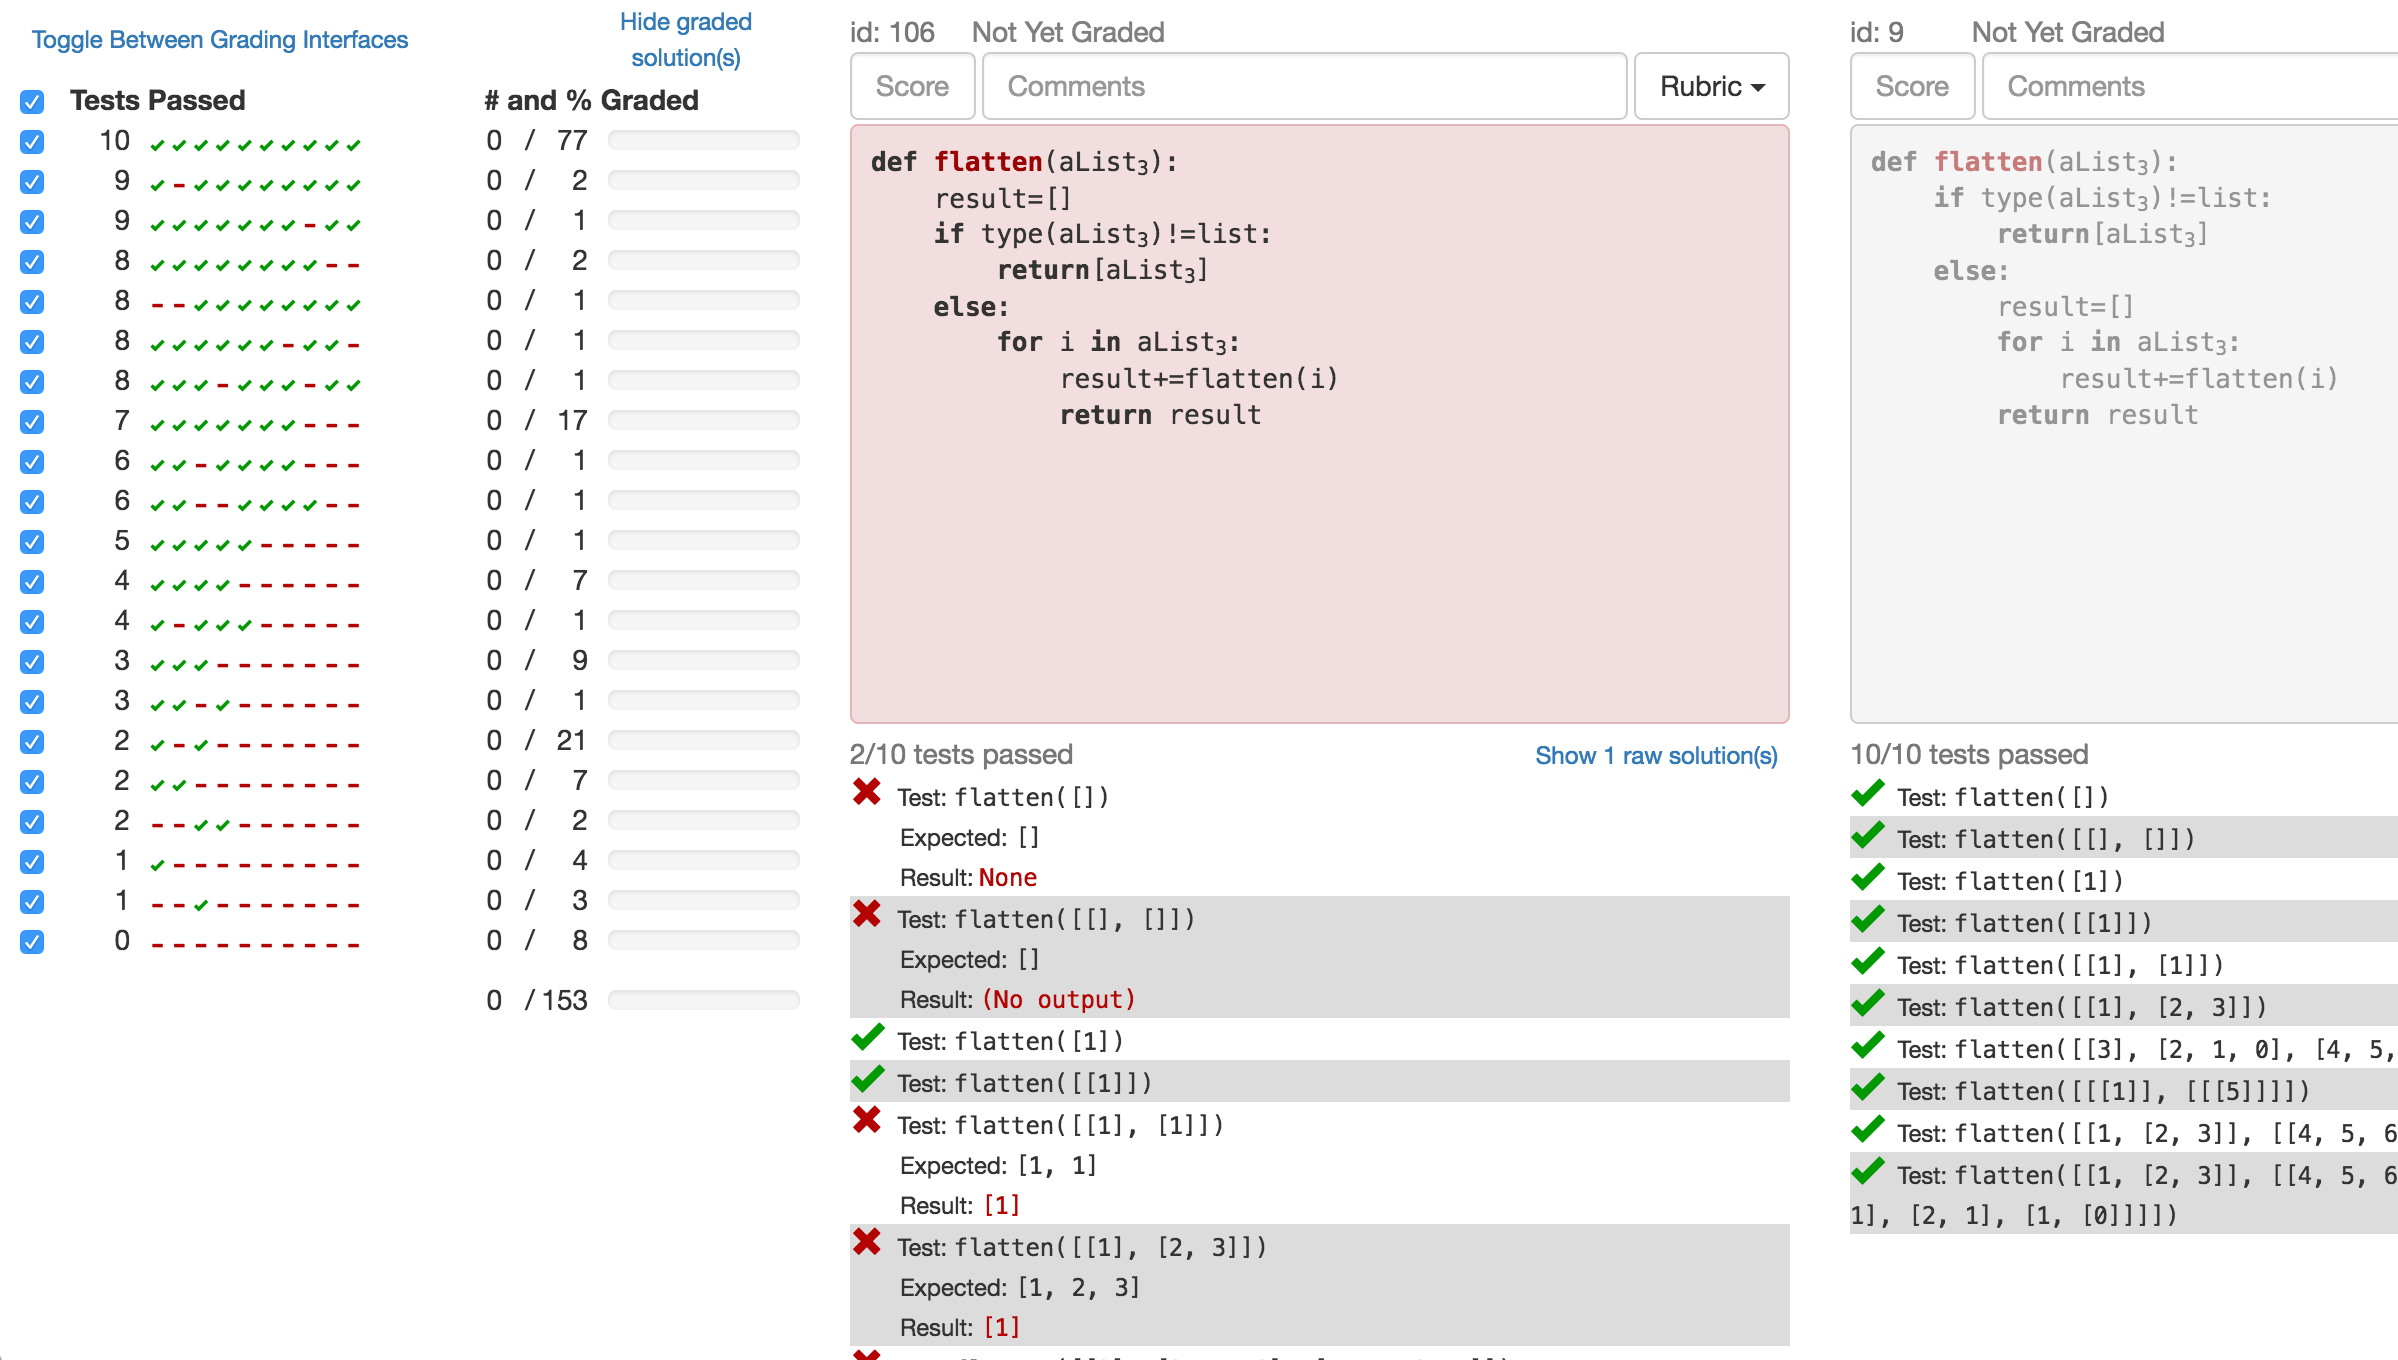
\includegraphics[width=\textwidth]{Body/figures/grovercode/figure_1}
\caption{The GroverCode user interface displaying solutions to an introductory Python programming exam problem, in which students are asked to implement a function to flatten a nested list of arbitrary depth.
}
\label{fig:whole_interface}
\end{figure} 

\begin{figure*}[t!]
    \centering
    \begin{subfigure}[b]{0.5\textwidth}
        \centering
        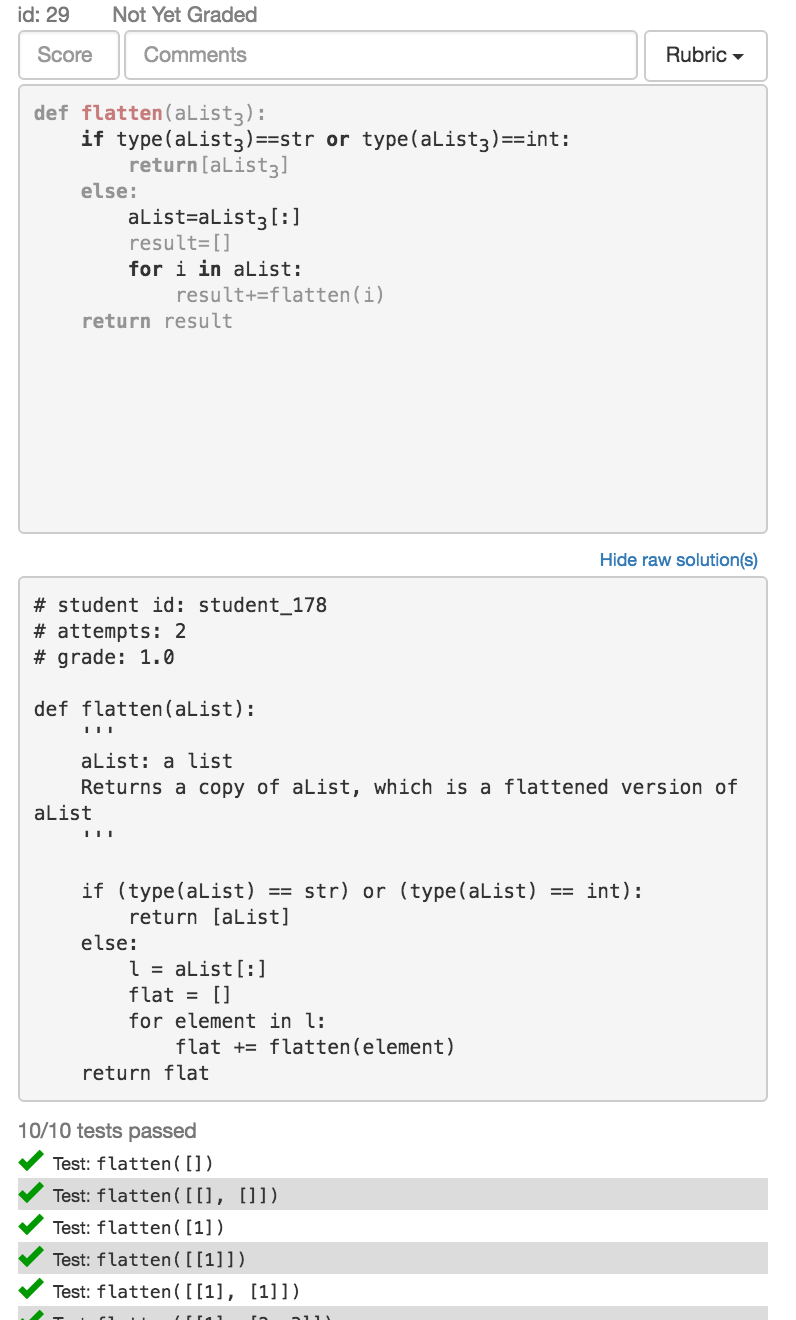
\includegraphics[height=4in]{Body/figures/grovercode/figure_2}
        \caption{A correct solution, its corresponding raw solution, and its performance on test cases, as displayed in GroverCode.}
        \label{fig:correct_stack}
    \end{subfigure}%
    ~ 
    \begin{subfigure}[b]{0.5\textwidth}
        \centering
        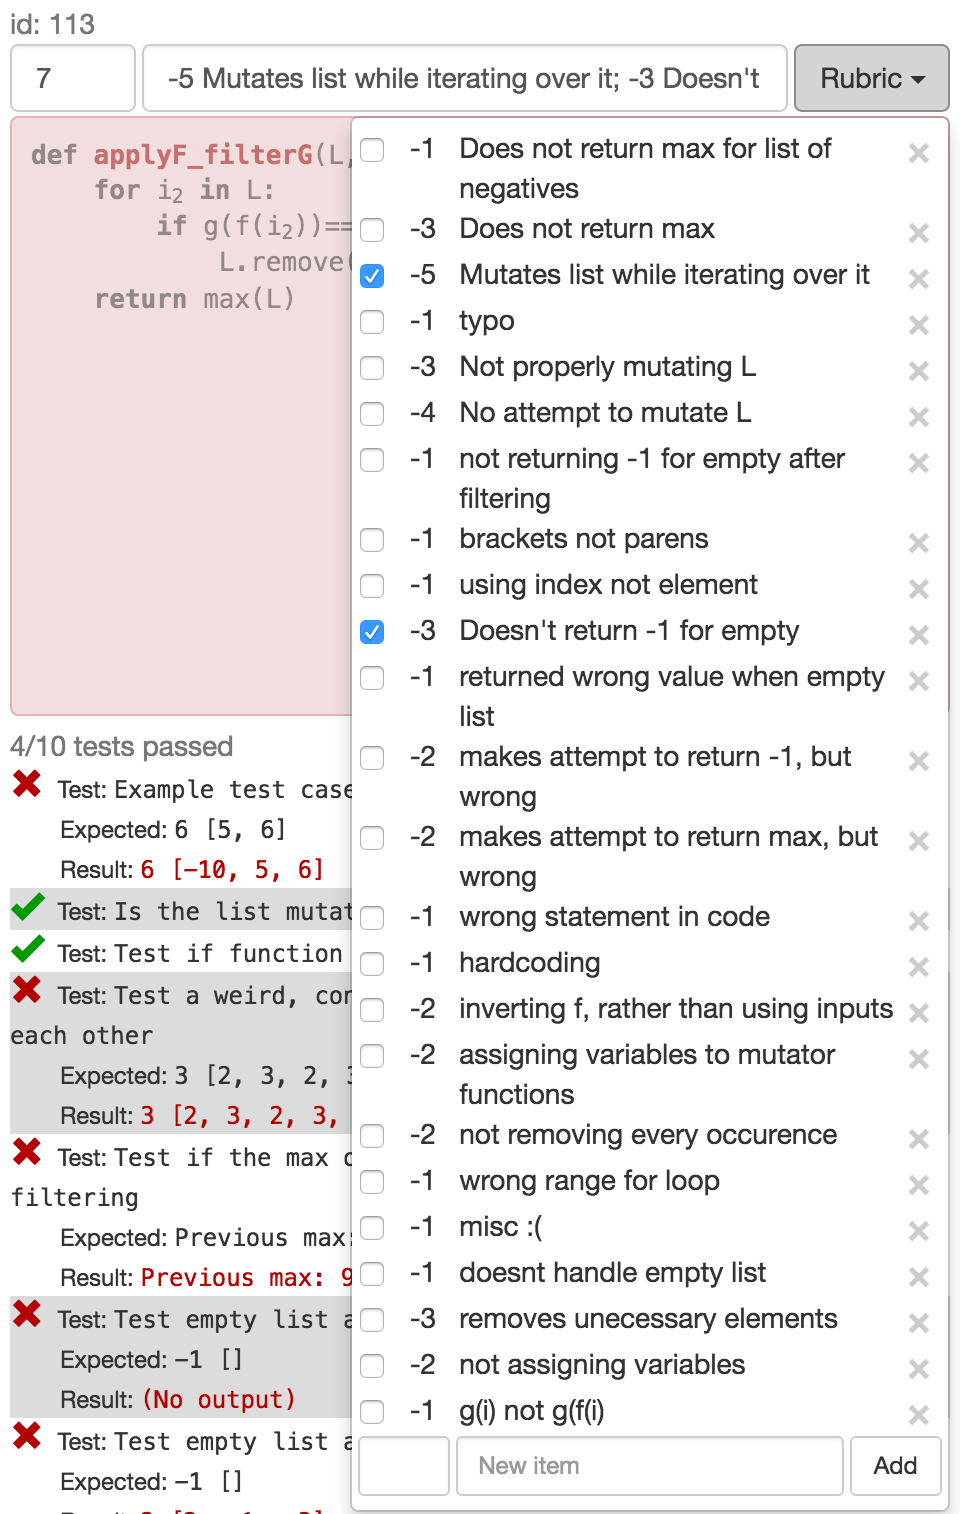
\includegraphics[height=4in]{Body/figures/grovercode/figure_3}
        \caption{An incorrect solution with the rubric dropdown menu open. Text for each of the checked items is automatically inserted in the comment box.}
        \label{fig:rubric}
    \end{subfigure}
    \caption{Correct and incorrect solutions, as rendered by GroverCode.}
\label{fig:correct_and_incorrect_stacks}
\end{figure*}

% \begin{figure}
% \centering
% 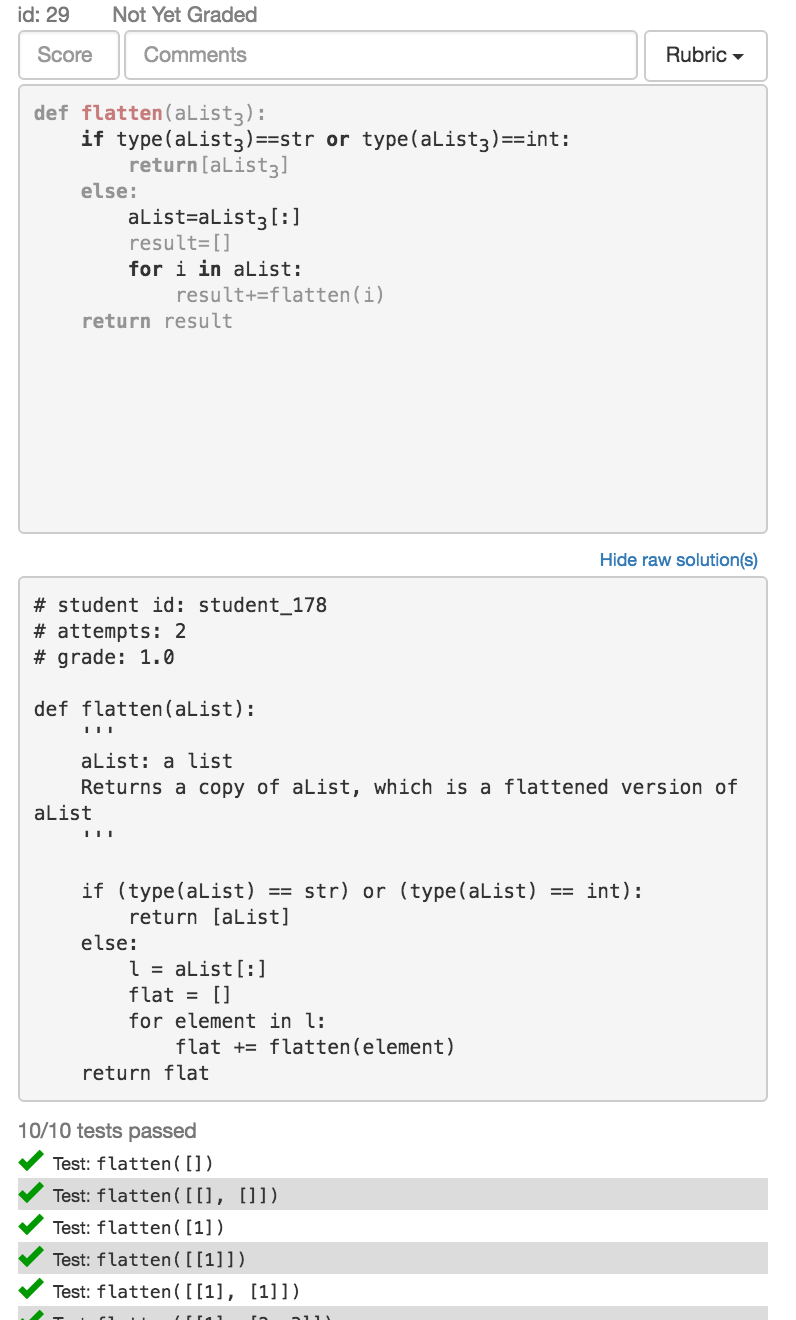
\includegraphics[width=0.5\textwidth]{Body/figures/grovercode/figure_2}
% \caption{A correct solution, its corresponding raw solution, and its performance on test cases, as displayed in GroverCode.}
% \label{fig:correct_stack}
% \end{figure}

% \begin{figure}
% \centering
% 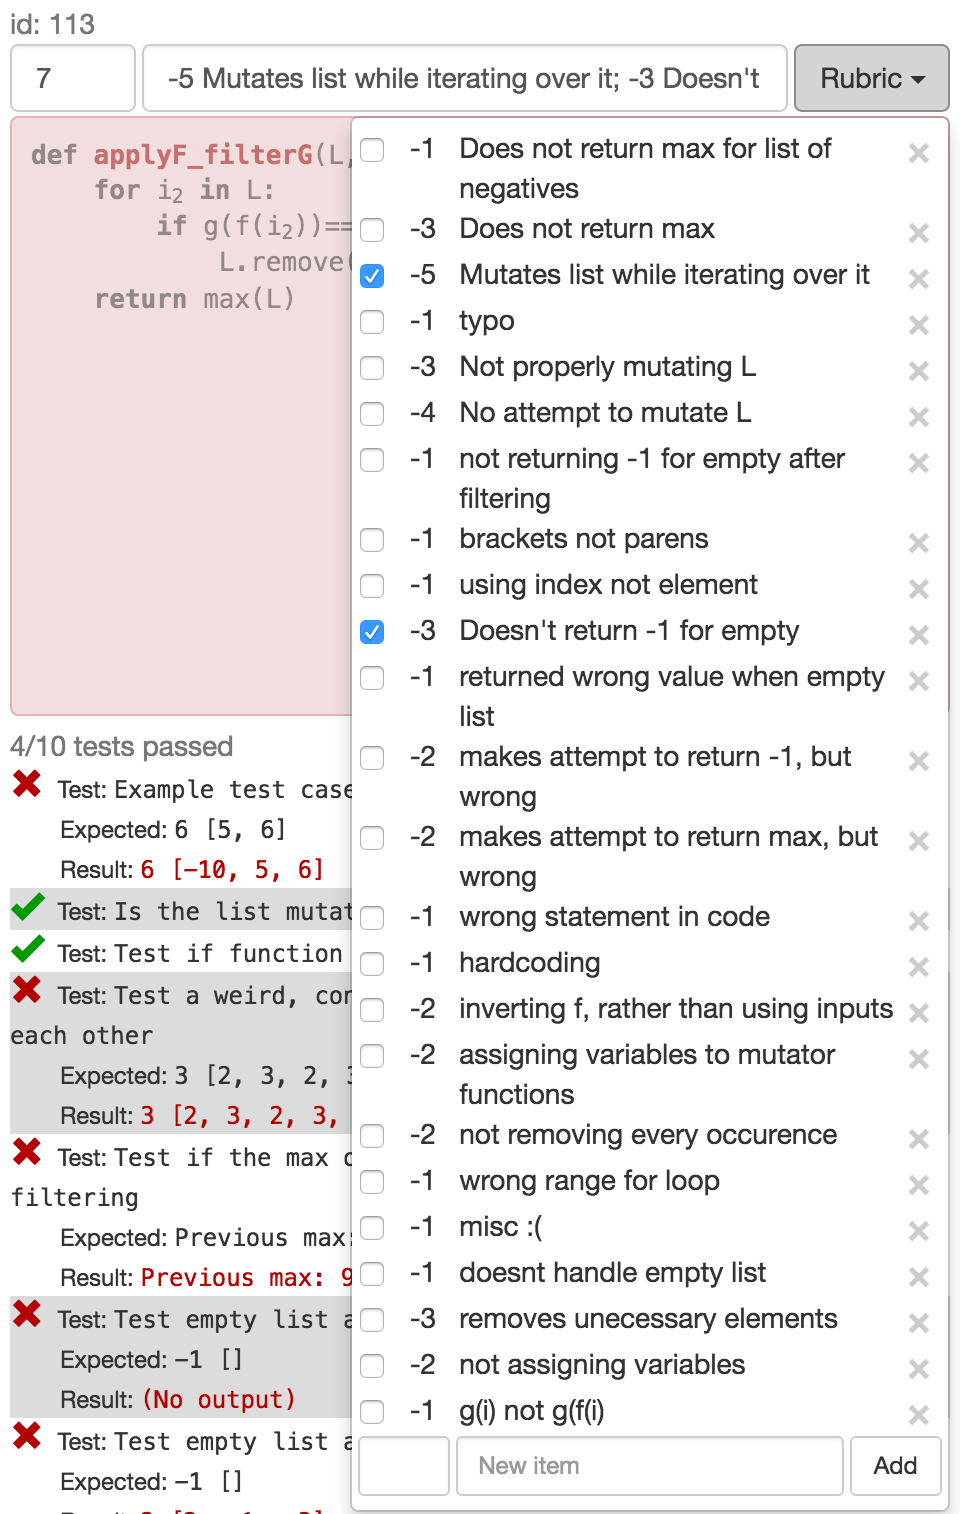
\includegraphics[width=0.5\textwidth]{Body/figures/grovercode/figure_3}
% \caption{A stack with the rubric dropdown menu open. Text for each of the checked items is automatically inserted in the comment box.}
% \label{fig:rubric}
% \end{figure}

The panel of progress indicators and filters, shown on the left side of Figure~\ref{fig:whole_interface}, helps teachers understand the distribution of solution behavior on test cases, track their grading progress, and grade sets of solutions that fail the same test cases one at a time. The rows of aligned sequences of green checks and red dashes represent error vectors, i.e., the pass/fail results with respect to the ordered list of teacher-specified test cases. The checkbox next to each error vector allows the teacher to selectively view subsets of solutions based on the particular tests they pass and fail. Solutions with the same error vectors may include similar mistakes. 

Like OverCode, GroverCode groups correct solutions into stacks. Grades are propagated to all the solutions in a stack. Incorrect solutions were not also grouped into stacks because the stacking process was new and experimental for field deployment in an actual grading session. GroverCode still normalized all solutions, both correct and incorrect.

The grading performed by the 6.0001 staff was intellectually demanding. For example, many staff members attempted to correct incorrect solutions by hand to better undertstand how far off the student was from a correct answer. When raw solutions are shown in random order, one solution may have a different approach, behavior, and appearance from the next. The transition from grading one solution to the next can mean starting from scratch. In an attempt to minimize the cognitive load of switching from one solution to the next, the GroverCode user interface includes the following features:
\begin{itemize}
\item Horizontally aligned solutions for side-by-side comparison
\item Easy filtering of solutions by input-output behavior, i.e., their error vectors
\item Normalized variable names
\item Solutions ordered to minimize the distance between adjacent solutions with respect to a custom similarity metric defined in Stacey Terman's Master's of Engineering thesis~\cite{staceythesis}
\item Highlighted lines of code in each solution which differ from the previous solution in the horizontal list
\end{itemize}

In OverCode, a single-line difference between two solutions could, by affecting a variable's behavior, cause the variable renaming process to propagate that difference as a variable name change throughout all the lines that mention the affected variable. This non-locality of difference made it harder to spot in the user interface where the actual syntactic difference between two platonic solutions was. As a result, stacks are rendered in the GroverCode user interface slightly differently. Even if the normalized variable names are different between two syntactically identical lines of code in two different stacks, if the variables take on the same sequence of values {\it just within that line of code}, it will not be highlighted as different in the user interface. Only the line with the syntactic difference will be highlighted.


\subsubsection{Implementation}~\label{subsec:grovercodepipeline}

The GroverCode implementation is a modification of the OverCode pipeline. Solutions which return an expected output for all test cases during the preprocessing step are categorized as correct, and all other solutions, having failed at least one test case, are categorized as incorrect. Correct solutions are normalized by the same process as was used in the original OverCode. 

In the original OverCode pipeline for correct solutions, variable behavior is assumed to hold enough semantic information to be the sole basis on which variable names are normalized. GroverCode applies this rule to incorrect solutions as well, but only for variables whose behavior matches a common variable in the correct solutions. This step may be error prone. Incorrect solutions are known to be wrong with respect to input-output behavior, the behavior of the variables within them is suspect too, even if it happens to match a common variable in a correct solution. %if a variable in an incorrect solution has the same behavior as a common variable in the correct solutions, GroverCode will rename the variable in the incorrect solution so it matches the common variable's name in the correct solutions.

%However, this renaming strategy may change in future versions of GroverCode because, 

In incorrect solutions, syntax, e.g., the operations applied to a variable, may be more helpful for normalizing variable names than behavior. For example, in an incorrect solution, a variable $i$ may be operated or depended on exactly the same way as a common variable in a correct solution. However, if an error somewhere else in the solution causes $i$ to behave differently, the original method of identifying common variables will be thrown off. %Based on this example, variables in incorrect solutions that are not already renamed based on behavior are renamed based on syntax.

The OverCode pipeline is modified for GroverCode to capture this syntactic information. The modified pipeline examines the program trace collected during preprocessing and the AST for each solution and compiles the following information for each line of code in each solution:
\begin{enumerate}
\item a template, i.e., the line of code with variables replaced by blanks, e.g., \texttt{\underline{\hspace{1em}} += 1} and \texttt{for \underline{\hspace{1em}} in range(\underline{\hspace{1em}}):}
\item an ordered list of the common variable behaviors and their normalized names corresponding to each blank in the line, e.g., the blank in \texttt{\underline{\hspace{1em}} += 1} can be associated with one of several common variables, depending on the rest of the solution
\item an ordered list of the sequences of values each blanked-out variable in the line took on during execution, e.g., the first blank in \texttt{for \underline{\hspace{1em}} in range(\underline{\hspace{1em}}):} might iterate through \texttt{1,2,3} while, with each visitation of this line during execution, the second blank stays constant at \texttt{[1,2,3],[1,2,3],[1,2,3]}
\end{enumerate}
Items 1 and 2 in this list together contain the information in the original normalized lines in OverCode and information about the line's syntax, regardless of the variables identities. Items 1 and 3 capture the information necessary to tell what the variable behavior is just within that one line and whether two lines in two different stacks will be highlighted as different from each other. This information is also used for variable renaming in incorrect solutions.

\begin{table}
\centering
%Copied with permission from Terman~\cite{staceythesis}}\todo{get explicit permission}
\begin{tabular}{l l r}
%\hline
 &  & {\bf Location} \\
{\bf Example line of code} & {\bf Template} & {\bf of \texttt{exp}} \\
\hline
\footnotesize{\texttt{def power(base, exp):}} & \footnotesize{\texttt{def power(\underline{\hspace{1em}}},\underline{\hspace{1em}}):} & 1 \\
%\hline
\footnotesize{\texttt{while index <= exp:}} & \footnotesize{\texttt{while \underline{\hspace{1em}}<=\underline{\hspace{1em}}:}} & 1 \\
%\hline
\footnotesize{\texttt{return 1.0*base*power(base, exp-1)}} & \footnotesize{\texttt{return 1.0*\underline{\hspace{1em}}*\underline{\hspace{1em}}*power(\underline{\hspace{1em}},\underline{\hspace{1em}}-1)}} & 3 \\
%\hline
\footnotesize{\texttt{return base*power(base, exp-1)}} & \footnotesize{\texttt{return \underline{\hspace{1em}}*power(\underline{\hspace{1em}},\underline{\hspace{1em}}-1)}} & 2 \\
%\hline
\footnotesize{\texttt{return power(base, exp-1)*base}} & \footnotesize{\texttt{return power(\underline{\hspace{1em}},\underline{\hspace{1em}}-1)*\underline{\hspace{1em}}}} & 1 \\
%\hline
\footnotesize{\texttt{ans = base*power(base, exp-1)}} & \footnotesize{\texttt{\underline{\hspace{1em}}=\underline{\hspace{1em}}*power(\underline{\hspace{1em}},\underline{\hspace{1em}}-1)}} & 3 \\
%\hline
\footnotesize{\texttt{if exp <= 0:}} & \footnotesize{\texttt{if \underline{\hspace{1em}}<=0:}} & 0 \\
%\hline
\footnotesize{\texttt{if exp == 0:}} & \footnotesize{\texttt{if \underline{\hspace{1em}}==0:}} & 0 \\
%\hline
\footnotesize{\texttt{if exp >= 1:}} & \footnotesize{\texttt{if \underline{\hspace{1em}} >= 1:}} & 0 \\
%\hline
\footnotesize{\texttt{assert type(exp) is int and exp >= 0}} & \footnotesize{\texttt{assert type(\underline{\hspace{1em}}) is int and \underline{\hspace{1em}}>=0}} & 0, 1 \\
%\hline
\end{tabular}
\caption{\textbf{Example:} All templates and locations in which the abstract variable \texttt{exp}, the second argument to a recursive \texttt{power} function, appears. A location represents the index or indices of the blanks that the abstract variable occupies, where the first blank is index 0, the second is index 1, and so on. The second and third columns together form a template-location pair.} 
\label{tab:templatelocation}
\end{table}

The GroverCode normalization process uses this syntactic information, in addition to behavior, to identify and rename common variables. The line's template, e.g., \texttt{for \underline{\hspace{1em}} in \underline{\hspace{1em}}:} is the syntax of the line with variable names removed. For each common variable in correct solutions, GroverCode counts how many times it appears in each template and in which location, represented as an index into the blanks in the template. Examples of templates and locations are shown in Table \autoref{tab:templatelocation}. If a yet-unrenamed variable in an incorrect solution appears in the exact same template-locations as a common variable in a correct solution, it will be renamed to match that common variable. If a variable in an incorrect solution is still not normalized, the counts of template-locations associated with each common variable in the correct solutions are used, as described in detail in Terman~\cite{staceythesis}, to infer the most likely common variable it could be renamed to, as long as a threshold for similarity is met. Otherwise, its original name is kept.





\subsubsection{Field Deployment}

Approximately two hundred students were enrolled in 6.0001, and nine instructors used GroverCode to grade nearly all student solutions. %Seven programming problems of a variety of difficulties were graded over the course of these two sessions.
The GroverCode analysis pipeline was run on both the midterm and final exam problems from the Spring 2016 semester of 6.0001, which had approximately 200 students enrolled. These exams contained seven programming problems in total, and between 133 and 189 solutions per problem made it through the analysis pipeline to be displayed in the user interface. The midterm problem prompts were:
\begin{itemize}
\item \texttt{power} (q4): Write a recursive function to calculate the exponential \texttt{base} to the power \texttt{exp}.
\item \texttt{give\_and\_take} (q5): Given a dictionary \texttt{d} and a list \texttt{L}, return a new dictionary that contains the keys of \texttt{d}. Map each key to its value in \texttt{d} plus one if the key is contained in \texttt{L}, and its value in d minus one if the key is not contained in \texttt{L}.
\item \texttt{closest\_power} (q6): Given an integer base and a target integer \texttt{num}, find the integer exponent that minimizes the difference between \texttt{num} and \texttt{base} to the power of exponent, choosing the smaller exponent in the case of a tie.
\end{itemize}
The final problem prompts were:
\begin{itemize}
\item \texttt{deep\_reverse} (q4): Write a function that takes a list of lists of integers \texttt{L}, and reverses \texttt{L} and each element of \texttt{L} in place.
\item \texttt{applyF\_filterG} (q5): Write a function that takes three arguments: a list of integers \texttt{L}, a function \texttt{f} that takes an integer and returns an integer, and a function \texttt{g} that takes an integer and returns a boolean. Remove elements from \texttt{L} such that for each remaining element \texttt{i}, \texttt{f(g(i))} returns \texttt{True}. Return the largest element of the mutated list, or -1 if the list is empty after mutation.
\item \texttt{MITCampus} (q6): Given the definitions of two classes: \texttt{Location}, which represents a two-dimensional coordinate point, and \texttt{Campus}, which represents a college campus centered at a particular \texttt{Location}, fill in several methods in the \texttt{MITCampus} class, a subclass of \texttt{Campus} that represents a college campus with tents at various \texttt{Locations}.
\item \texttt{longest\_run} (q7): Write a function that takes a list of integers \texttt{L}, finds the longest run of either monotonically increasing or monotonically decreasing integers in \texttt{L}, and returns the sum of this run.
\end{itemize}
For each problem processed during the field deployments, an example of a staff-written correct solution is included in the Appendix.

Using the GroverCode user interface, nine instructors, including one lecturer and eight teaching assistants (TAs) graded these solutions as part of their official grading responsibilities. Stacey Terman, the Master's of Engineering student who implemented most of GroverCode, was one of these TAs. Solutions that did not successfully pass through the pipeline were graded by hand afterwards. TA grading events, e.g., adding or applying rubric items and point values to solutions, were logged. The observer (the author of this thesis) took extensive notes during each day-long grading session to capture spontaneous feature requests as well as bugs and complaints. 

%\begin{comment}
% {\bf Programming Exam Problems}

%Given the increasing difficulty of these exam problems, the following numbers dropped between the midterm and the final: the number of students present to take the exam, the number of students who submitted any solution to a given problem before the test period ended, and the number of correct solutions that could be clustered.

\subsubsection{Pipeline Evaluation}

The number of solutions submitted for each problem and the number that were successfully processed by the GroverCode pipeline is shown in Table~\ref{table:num_submissions}. Table~\ref{table:cluster_stats} captures the scale of the variation as well as some clustering statistics. Table~\ref{table:renametype} summarizes the counts of the various mechanims by which variables in incorrect solutions were normalized.

\begin{table}[h!]
\centering
\begin{tabular}{l r|r|r|r|r|r|r}
%\hline
& \multicolumn{3}{c}{Quiz} & \multicolumn{4}{c}{Final} \\
%\cline{2-8}
& q4 & q5 & q6 & q4 & q5 & q6 & q7 \\
\hline
Submissions & 193 & 193 & 193 & 175 & 173 & 170 & 165 \\
\hline
Mean lines per solution & 9.9 & 16.9 & 19.8 & 12.3 & 20.9 & 50.0 & 41.8 \\
\hline
Solutions & 186 & 189 & 168  & 170 & 166  & 134 & 133 \\
successfully processed & 96\% & 98\% & 87\% & 97\% & 96\% & 79\% & 81\% \\
%\hline
\end{tabular}
\caption{Number of solutions submitted and successfully processed by GroverCode for each problem in the dataset. Reasons why a solution might not make it through the pipeline include syntax errors and memory management issues caused by students' inappropriate function calls.}
\label{table:num_submissions}
\end{table}

\begin{table}[!ht]
\centering
\begin{tabular}{l r|r|r|r|r|r|r}
%\hline
& \multicolumn{3}{c}{Quiz} & \multicolumn{4}{c}{Final} \\
%\cline{2-8}
& q4 & q5 & q6 & q4 & q5 & q6 & q7 \\
\hline
Correct solutions & 182 & 160 & 94 & 96 & 49 & 16 & 12 \\
 & 94\% & 82\% & 49\% & 55\% & 28\% & 9\% & 7\% \\
\hline
Incorrect solutions & 4 & 29 & 74 & 74 & 117 & 118 & 121 \\
\hline
Test cases & 10 & 15 & 25 & 11 & 10 & 17 & 28 \\
\hline
Distinct error signatures & 6 & 16 & 36 & 12 & 38 & 57 & 42 \\
\hline
Correct stacks & 40 & 84 & 93 & 47 & 46 & 16 & 12 \\
\hline
Stacks with > 1 solution & 13 & 18 & 1 & 8 & 2 & 0 & 0 \\
\hline
Solutions in stacks & 151 & 94 & 2 & 57 & 5 & 0 & 0 \\
%\hline
\end{tabular}
\caption{The degree of variation in input-output behavior and statistics about stack sizes.}
\label{table:cluster_stats}
\end{table}

\begin{table}
\centering
\begin{tabular}{l c|c|c|c|c|c|c}
%\hline
& \multicolumn{3}{c}{Quiz} & \multicolumn{4}{c}{Final} \\
%\cline{2-8}
& q4 & q5 & q6 & q4 & q5 & q6 & q7 \\
\hline
Variables in incorrect submissions & 15 & 149 & 482 & 289 & 550 & 559 & 859 \\
\hline
Variables renamed based on values & 14 & 84 & 266 & 97 & 246 & 97 & 187 \\
\hline
Variables renamed based on templates & 0 & 58 & 166 & 136 & 264 & 188 & 489 \\
\hline
Variables not renamed & 1 & 7 & 50 & 56 & 40 & 274 & 183 \\
%\hline
\end{tabular}
\caption{Statistics about variables renaming based on different heuristics in the GroverCode normalization process.}
\label{table:renametype}
\end{table}
%\end{comment}
 
\subsubsection{Discussion}

GroverCode was particularly appreciated on simpler problems where correct solutions were clustered together and graded by a single action. Under these conditions, the clustering capability GroverCode inherits from OverCode amplified teacher effort.

Variable renaming was, for simpler programming problems, an invisible and possibly slightly confusing helping hand. One grader remarked, out loud: ``Why is everyone naming their iterator variable `i'?'' at which point he had to be reminded of the variable renaming process. 

When applied to more complex solutions, the normalization process was at times more harmful than helpful for teacher comprehension. As solutions became more varied and structurally complex, graders started toggling off normalization because the renaming of variables, removal of comments, and formatting standardization was removing clues they needed in order to understand student intent.

The feature for grouping solutions based on their behavior on test cases was appreciated regardless of solution complexity. While it was difficult to get direct feedback on the helpfulness of pair-wise difference highlighting and optimized solution ordering, graders heavily used and appreciated the ability to filter and grade solutions one error vector at a time. At least one grader remarked aloud that it seemed like many of the solution with the same error vector made similar mistakes. Therefore filtering by error vector may have been one of the stronger contributors to any hypothetical decreased cognitive load due to using GroverCode over the status quo of random assignment to solutions in a CSV file.

%\todo{DNHT: add to related work Appropriately chosen latent variable models have already been used in the past to model open-source code and answers to open-response mathematical questions.}

\section{Conclusion}
OverCode is a novel system for visualizing thousands of Python programming solutions that helps teachers explore the variations among them. Unlike previous approaches, OverCode uses a lightweight static and dynamic analysis to generate platonic solutions that represent stacks of similar solutions in an interactive user interface. It allows teachers to filter stacks by normalized lines of code and to further merge different stacks by composing rewrite rules. As observed in two user studies with a total of 24 current and potential teaching assistants, OverCode allowed teachers to more quickly develop a high-level view of students' understanding and misconceptions, and provide feedback that is relevant to more student solutions. 

GroverCode, an extension of OverCode which handles incorrect solutions, is a new tool for triaging and hand-grading solutions. It was successfully deployed in the field as the tool for grading the midterm and final exams of MIT's 6.0001 course, ``Introduction to Computer Science and Programming in Python''. Based on teachers' appreciation of the interface over the existing alternatives, GroverCode will continue to be deployed in the field to ease the subjective psychological burden of grading hundreds of Python programs. %I believe an information visualization approach is necessary for teachers to explore the variations among solutions at the scale of MOOCs, and OverCode is an important step towards that goal.
%\todo{make sure evidence of teacher's appreciate is included}